%\documentclass[10pt,handout]{beamer}
\documentclass[10pt]{beamer}
\usepackage[english]{babel} % Anpassa efter svenska. Ger svensk logga.
\usepackage[utf8]{inputenc} % Anpassa efter linux
\usepackage{graphicx}
\usepackage{hyperref}
\usepackage{listings}
\lstdefinelanguage{Stan}{
  morekeywords=[1]{functions,data,parameters,transformed,model,generated,quantities,%
    for,in,while,print,if,else,lower,upper,increment_log_prob,T,return,%
    reject,integrate_ode,integrate_ode_bdf,integrate_ode_rk45,target},%
  morekeywords=[2]{int,real,vector,%
    ordered,positive_ordered,simplex,unit_vector,%
    row_vector,matrix,%
    cholesky_factor_corr,cholesky_factor_cov,%
    coor_matrix,cov_matrix,%
    void},%
  morekeywords=[3]{%
    Phi,%
    Phi_approx,%
    abs,%
    acos,%
    acosh,%
    append_col,%
    append_row,%
    asin,%
    asinh,%
    atan,%
    atan2,%
    atanh,%
    bernoulli_cdf,%
    bernoulli_cdf_log,%
    bernoulli_lccdf,%
    bernoulli_lcdf,%
    bernoulli_logit_lpmf,%
    bernoulli_logit_lpmf,%
    bernoulli_lpmf,%
    bernoulli_lpmf,%
    bernoulli_rng,%
    bessel_first_kind,%
    bessel_second_kind,%
    beta_binomial_cdf,%
    beta_binomial_cdf_log,%
    beta_binomial_lccdf,%
    beta_binomial_lcdf,%
    beta_binomial_lpmf,%
    beta_binomial_lpmf,%
    beta_binomial_rng,%
    beta_cdf,%
    beta_cdf_log,%
    beta_lccdf,%
    beta_lcdf,%
    beta_lpdf,%
    beta_lpdf,%
    beta_rng,%
    binary_log_loss,%
    binomial_cdf,%
    binomial_cdf_log,%
    binomial_coefficient_log,%
    binomial_lccdf,%
    binomial_lcdf,%
    binomial_logit_lpmf,%
    binomial_logit_lpmf,%
    binomial_lpmf,%
    binomial_lpmf,%
    binomial_rng,%
    block,%
    categorical_logit_lpmf,%
    categorical_logit_lpmf,%
    categorical_lpmf,%
    categorical_lpmf,%
    categorical_rng,%
    cauchy_cdf,%
    cauchy_cdf_log,%
    cauchy_lccdf,%
    cauchy_lcdf,%
    cauchy_lpdf,%
    cauchy_lpdf,%
    cauchy_rng,%
    cbrt,%
    ceil,%
    chi_square_cdf,%
    chi_square_cdf_log,%
    chi_square_lccdf,%
    chi_square_lcdf,%
    chi_square_lpdf,%
    chi_square_lpdf,%
    chi_square_rng,%
    cholesky_decompose,%
    col,%
    cols,%
    columns_dot_product,%
    columns_dot_self,%
    cos,%
    cosh,%
    crossprod,%
    csr_extract_u,%
    csr_extract_v,%
    csr_extract_w,%
    csr_matrix_times_vector,%
    csr_to_dense_matrix,%
    cumulative_sum,%
    determinant,%
    diag_matrix,%
    diag_post_multiply,%
    diag_pre_multiply,%
    diagonal,%
    digamma,%
    dims,%
    dirichlet_lpdf,%
    dirichlet_lpdf,%
    dirichlet_rng,%
    distance,%
    dot_product,%
    dot_self,%
    double_exponential_cdf,%
    double_exponential_cdf_log,%
    double_exponential_lccdf,%
    double_exponential_lcdf,%
    double_exponential_lpdf,%
    double_exponential_lpdf,%
    double_exponential_rng,%
    e,%
    eigenvalues_sym,%
    eigenvectors_sym,%
    erf,%
    erfc,%
    exp,%
    exp2,%
    exp_mod_normal_cdf,%
    exp_mod_normal_cdf_log,%
    exp_mod_normal_lccdf,%
    exp_mod_normal_lcdf,%
    exp_mod_normal_lpdf,%
    exp_mod_normal_lpdf,%
    exp_mod_normal_rng,%
    expm1,%
    exponential_cdf,%
    exponential_cdf_log,%
    exponential_lccdf,%
    exponential_lcdf,%
    exponential_lpdf,%
    exponential_lpdf,%
    exponential_rng,%
    fabs,%
    falling_factorial,%
    fdim,%
    floor,%
    fma,%
    fmax,%
    fmin,%
    fmod,%
    frechet_cdf,%
    frechet_cdf_log,%
    frechet_lccdf,%
    frechet_lcdf,%
    frechet_lpdf,%
    frechet_lpdf,%
    frechet_rng,%
    gamma_cdf,%
    gamma_cdf_log,%
    gamma_lccdf,%
    gamma_lcdf,%
    gamma_lpdf,%
    gamma_lpdf,%
    gamma_p,%
    gamma_q,%
    gamma_rng,%
    gaussian_dlm_obs_lpdf,%
    gaussian_dlm_obs_lpdf,%
    get_lp,%
    gumbel_cdf,%
    gumbel_cdf_log,%
    gumbel_lccdf,%
    gumbel_lcdf,%
    gumbel_lpdf,%
    gumbel_lpdf,%
    gumbel_rng,%
    head,%
    hypergeometric_lpmf,%
    hypergeometric_lpmf,%
    hypergeometric_rng,%
    hypot,%
    if_else,%
    inc_beta,%
    int_step,%
    inv,%
    inv_chi_square_cdf,%
    inv_chi_square_cdf_log,%
    inv_chi_square_lccdf,%
    inv_chi_square_lcdf,%
    inv_chi_square_lpdf,%
    inv_chi_square_lpdf,%
    inv_chi_square_rng,%
    inv_cloglog,%
    inv_gamma_cdf,%
    inv_gamma_cdf_log,%
    inv_gamma_lccdf,%
    inv_gamma_lcdf,%
    inv_gamma_lpdf,%
    inv_gamma_lpdf,%
    inv_gamma_rng,%
    inv_logit,%
    inv_phi,%
    inv_sqrt,%
    inv_square,%
    inv_wishart_lpdf,%
    inv_wishart_lpdf,%
    inv_wishart_rng,%
    inverse,%
    inverse_spd,%
    is_inf,%
    is_nan,%
    lbeta,%
    lchoose,%
    lgamma,%
    lkj_corr_cholesky_lpdf,%
    lkj_corr_cholesky_lpdf,%
    lkj_corr_cholesky_rng,%
    lkj_corr_lpdf,%
    lkj_corr_lpdf,%
    lkj_corr_rng,%
    lmgamma,%
    lmultiply,%
    log,%
    log10,%
    log1m,%
    log1m_exp,%
    log1m_inv_logit,%
    log1p,%
    log1p_exp,%
    log2,%
    log_determinant,%
    log_diff_exp,%
    log_falling_factorial,%
    log_inv_logit,%
    log_mix,%
    log_rising_factorial,%
    log_softmax,%
    log_sum_exp,%
    logistic_cdf,%
    logistic_cdf_log,%
    logistic_lccdf,%
    logistic_lcdf,%
    logistic_lpdf,%
    logistic_lpdf,%
    logistic_rng,%
    logit,%
    lognormal_cdf,%
    lognormal_cdf_log,%
    lognormal_lccdf,%
    lognormal_lcdf,%
    lognormal_lpdf,%
    lognormal_lpdf,%
    lognormal_rng,%
    machine_precision,%
    max,%
    mdivide_left_tri_low,%
    mdivide_right_tri_low,%
    mean,%
    min,%
    modified_bessel_first_kind,%
    modified_bessel_second_kind,%
    multi_gp_cholesky_lpdf,%
    multi_gp_cholesky_lpdf,%
    multi_gp_lpdf,%
    multi_gp_lpdf,%
    multi_normal_cholesky_lpdf,%
    multi_normal_cholesky_lpdf,%
    multi_normal_cholesky_rng,%
    multi_normal_lpdf,%
    multi_normal_lpdf,%
    multi_normal_prec_lpdf,%
    multi_normal_prec_lpdf,%
    multi_normal_rng,%
    multi_student_t_lpdf,%
    multi_student_t_lpdf,%
    multi_student_t_rng,%
    multinomial_lpmf,%
    multinomial_lpmf,%
    multinomial_rng,%
    multiply_log,%
    multiply_lower_tri_self_transpose,%
    neg_binomial_2_cdf,%
    neg_binomial_2_cdf_log,%
    neg_binomial_2_lccdf,%
    neg_binomial_2_lcdf,%
    neg_binomial_2_log_lpmf,%
    neg_binomial_2_log_lpmf,%
    neg_binomial_2_log_rng,%
    neg_binomial_2_lpmf,%
    neg_binomial_2_lpmf,%
    neg_binomial_2_rng,%
    neg_binomial_cdf,%
    neg_binomial_cdf_log,%
    neg_binomial_lccdf,%
    neg_binomial_lcdf,%
    neg_binomial_lpmf,%
    neg_binomial_lpmf,%
    neg_binomial_rng,%
    negative_infinity,%
    normal_cdf,%
    normal_cdf_log,%
    normal_lccdf,%
    normal_lcdf,%
    normal_lpdf,%
    normal_lpdf,%
    normal_rng,%
    not_a_number,%
    num_elements,%
    ordered_logistic_lpmf,%
    ordered_logistic_lpmf,%
    ordered_logistic_rng,%
    owens_t,%
    pareto_cdf,%
    pareto_cdf_log,%
    pareto_lccdf,%
    pareto_lcdf,%
    pareto_lpdf,%
    pareto_lpdf,%
    pareto_rng,%
    pareto_type_2_cdf,%
    pareto_type_2_cdf_log,%
    pareto_type_2_lccdf,%
    pareto_type_2_lcdf,%
    pareto_type_2_lpdf,%
    pareto_type_2_lpdf,%
    pareto_type_2_rng,%
    pi,%
    poisson_cdf,%
    poisson_cdf_log,%
    poisson_lccdf,%
    poisson_lcdf,%
    poisson_log_lpmf,%
    poisson_log_lpmf,%
    poisson_log_rng,%
    poisson_lpmf,%
    poisson_lpmf,%
    poisson_rng,%
    positive_infinity,%
    pow,%
    prod,%
    qr_Q,%
    qr_R,%
    quad_form,%
    quad_form_diag,%
    quad_form_sym,%
    rank,%
    rayleigh_cdf,%
    rayleigh_cdf_log,%
    rayleigh_lccdf,%
    rayleigh_lcdf,%
    rayleigh_lpdf,%
    rayleigh_lpdf,%
    rayleigh_rng,%
    rep_array,%
    rep_matrix,%
    rep_row_vector,%
    rep_vector,%
    rising_factorial,%
    round,%
    row,%
    rows,%
    rows_dot_product,%
    rows_dot_self,%
    scaled_inv_chi_square_cdf,%
    scaled_inv_chi_square_cdf_log,%
    scaled_inv_chi_square_lccdf,%
    scaled_inv_chi_square_lcdf,%
    scaled_inv_chi_square_lpdf,%
    scaled_inv_chi_square_lpdf,%
    scaled_inv_chi_square_rng,%
    sd,%
    segment,%
    sin,%
    singular_values,%
    sinh,%
    size,%
    skew_normal_cdf,%
    skew_normal_cdf_log,%
    skew_normal_lccdf,%
    skew_normal_lcdf,%
    skew_normal_lpdf,%
    skew_normal_lpdf,%
    skew_normal_rng,%
    softmax,%
    sort_asc,%
    sort_desc,%
    sort_indices_asc,%
    sort_indices_desc,%
    sqrt,%
    sqrt2,%
    square,%
    squared_distance,%
    step,%
    student_t_cdf,%
    student_t_cdf_log,%
    student_t_lccdf,%
    student_t_lcdf,%
    student_t_lpdf,%
    student_t_lpdf,%
    student_t_rng,%
    sub_col,%
    sub_row,%
    sum,%
    tail,%
    tan,%
    tanh,%
    tcrossprod,%
    tgamma,%
    to_array_1d,%
    to_array_2d,%
    to_matrix,%
    to_row_vector,%
    to_vector,%
    trace,%
    trace_gen_quad_form,%
    trace_quad_form,%
    trigamma,%
    trunc,%
    uniform_cdf,%
    uniform_cdf_log,%
    uniform_lccdf,%
    uniform_lcdf,%
    uniform_lpdf,%
    uniform_lpdf,%
    uniform_rng,%
    variance,%
    von_mises_lpdf,%
    von_mises_lpdf,%
    von_mises_rng,%
    weibull_cdf,%
    weibull_cdf_log,%
    weibull_lccdf,%
    weibull_lcdf,%
    weibull_lpdf,%
    weibull_lpdf,%
    weibull_rng,%
    wiener_lpdf,%
    wiener_lpdf,%
    wishart_lpdf,%
    wishart_lpdf,%
    wishart_rng
  },%
  otherkeywords={<-,~,+=,=},%
  sensitive=true,%
  morecomment=[l]{\#},%
  morecomment=[l]{//},%
  morecomment=[n]{/*}{*/},%
  string=[d]"%,
  literate={<-}{{$\leftarrow$}}1 {~}{{$\sim$}}1%
}
 % Stan listing[language=Stan]

\hypersetup{
    colorlinks=true,
    linkcolor=blue,
    filecolor=magenta,
    urlcolor=cyan,
}
\usepackage{../common/beamerthemeUppsala}
%\usetheme{Uppsala}
%\usecolortheme{UU} % Anpassa efter UU:s frger och logga
%\hypersetup{pdfpagemode=FullScreen} % Adobe Reader ska ppna fullskrm
\setbeamertemplate{itemize items}[circle]

% \usepackage{beamerthemesplit}
\usepackage{amsmath}
% \usepackage{amssymb}
% \usepackage{graphics}
% \usepackage{graphicx}
% \usepackage{epsfig}
% \usepackage[latin1]{inputenc}
 \usepackage{color}
% \usepackage{fancybox}
% \usepackage{psfrag}
% \usepackage[english]{babel}
 \setbeamertemplate{footline}{\hfill\insertframenumber/\inserttotalframenumber}

% Input new commands
%\usepackage{bm}
%\usepackage{natbib}
\newcommand{\bfm}[1]   {\mbox{\boldmath{${#1}$}}}
\newcommand{\Prob}   {\mbox{\textnormal{P}}}
\def\eqd{\,{\buildrel d \over =}\,}

% Vector/Matrix definitions (in bold type)
\newcommand{\vect}[1]{\mathbf{#1}}
\newcommand{\vectb}[1]{\bm{#1}}

% Differential operator 'd' as upright as in (use \dd)
\newcommand{\dd}{\; \mathrm{d}}

% Gaussian normal distribution (use \N)
\newcommand{\N}{\mathcal{N}} %% or \mathrm{N}

% Uniform distribution (use \Uni or \U)
\newcommand{\Uni}{\mathcal{U}} %% or \mathrm{U}
\newcommand{\U}{\mathcal{U}} %% or \mathrm{U}

% Matrix transpose (use \T)
\newcommand{\T}{^{\mathsf{T}}}

% Blockdiagonal matrices (use \blockdiag)
\newcommand{\blockdiag}{\mathrm{blockdiag}}

% Define inner product '<f,g>' notation (use \innerp{#1})
\providecommand{\innerp}[1]{\left\langle#1\right\rangle}

\def\o{{\mathbf o}}
\def\t{{\mathbf \theta}}
\def\w{{\mathbf w}}
\def\x{{\mathbf x}}
\def\y{{\mathbf y}}
\def\z{{\mathbf z}}



% Other math symbols and notation
\newcommand{\D}{^\mathsf{\dagger}}
\newcommand{\R}{\mathbb{R}}
\newcommand{\erf}{\mathrm{erf}}
\newcommand{\E}{\mathrm{E}}
\newcommand{\var}{\mathrm{var}}
\newcommand{\Var}{\mathrm{Var}}
\newcommand{\cov}{\mathrm{cov}}
\newcommand{\Ker}{\operatorname{Ker}}
\newcommand{\Ran}{\operatorname{Ran}}
\providecommand{\norm}[1]{\lVert#1\rVert}
\providecommand{\op}[1]{\mathcal{#1}}
\newcommand{\arccot}{\mathrm{arccot}}
\providecommand{\Hspace}[1]{\mathscr{#1}}
\providecommand{\fourier}[1]{\mathscr{#1}}

\newcommand{\kin}{k^{\rm in}}
\newcommand{\kout}{k^{\rm out}}
\newcommand{\gi}{{R_0}}
\newcommand{\eff}{{E_{\rm max}}}
\newcommand{\ESS}{\mathrm{ESS}}
\newcommand{\HN}{{\rm N^+}}
\newcommand{\lN}{{\rm LN}}

\DeclareMathOperator{\Sd}{Sd}
\DeclareMathOperator{\sd}{sd}
\DeclareMathOperator{\Gammad}{Gamma}
\DeclareMathOperator{\Invgamma}{Inv-gamma}
\DeclareMathOperator{\Bin}{Bin}
\DeclareMathOperator{\Negbin}{Neg-bin}
\DeclareMathOperator{\Poisson}{Poisson}
\DeclareMathOperator{\Beta}{Beta}
\DeclareMathOperator{\logit}{logit}
\DeclareMathOperator{\BF}{BF}
\DeclareMathOperator{\Invchi2}{Inv-\chi^2}
\DeclareMathOperator{\NInvchi2}{N-Inv-\chi^2}
\DeclareMathOperator{\InvWishart}{Inv-Wishart}
\DeclareMathOperator{\tr}{tr}
% \DeclareMathOperator{\Pr}{Pr}
\def\euro{{\footnotesize \EUR\, }}
\DeclareMathOperator{\rep}{\mathrm{rep}}


%%%%%%%%%%%%%%%%%%%%%%%%%%%%%%%%%%%%%%%%%%%%%%%%%%%%%%%%%%%%%%%%%%

\setlength{\parskip}{3mm}
\title[]{{\color{black}Bayesian Statistics and Data Analysis \\ Lecture 5}}
\author[]{M{\aa}ns Magnusson \\ Department of Statistics, Uppsala University \\ Thanks to Aki Vehtari, Aalto University}
\date{}

\begin{document}

\frame{\titlepage
% \thispagestyle{empty}
}

%%%%%%%%%%%%%%%%%%%%%%%%%%%%%%%%%%%%%%%%%%%%%%%%%%%%%%%%%%%%%%%%%%


\section{Monte Carlo recap}
%\frame{\sectionpage}


\begin{frame}

\frametitle{ It's all about expectations}

  \vspace{-1.5\baselineskip}
   \begin{align*}
     E_{\color{blue} p(\theta|y)}[f(\theta)] & = \int f(\theta) {\color{blue} p(\theta|y)} d\theta,\\
     \text{where} \quad
     {\color{blue} p(\theta|y)} & = \frac{\color{uured}p(y|\theta)p(\theta)}{\color{red} \int p(y|\theta)p(\theta) d\theta}
   \end{align*}
     \uncover<2->{We can easily evaluate ${\color{uured} p(y|\theta)p(\theta)}$ for any $\theta$, but the integral ${\color{red} \int p(y|\theta)p(\theta) d\theta}$ is usually difficult.}

   \uncover<3->{We can use the unnormalized posterior ${\color{uured} q(\theta|y)
     = p(y|\theta)p(\theta)}$, for example, in}
 \begin{itemize}
   \vspace{-0.5\baselineskip}
%    \item<4-> Grid (equal spacing) evaluation with self-normalization
%      \begin{align*}
%        E_{\color{blue} p(\theta|y)}[f(\theta)] \approx
%        \frac{\sum_{s=1}^S \left[f(\theta^{(s)}){\color{uured}q(\theta^{(s)}|y)}\right]}{\sum_{s=1}^S{\color{uured}q(\theta^{(s)}|y)}}
%      \end{align*}
    \item<4-> Monte Carlo methods which can sample from
      ${\color{blue}p(\theta^{(s)}|y)}$ using only
      ${\color{uured}q(\theta^{(s)}|y)}$
         \vspace{-0.5\baselineskip}
      \begin{align*}
        E_{\color{blue} p(\theta|y)}[f(\theta)] \approx \frac{1}{S} \sum_{s=1}^S f(\theta^{(s)})
      \end{align*}
    \end{itemize}

\end{frame}


\begin{frame}

\frametitle{ Monte Carlo}

  \begin{itemize}
  \item Monte Carlo methods we have discussed so far
    \begin{itemize}
    \item Inverse CDF works for 1D \pause
    \item Analytic transformations work for only certain distributions \pause
%    \item Factorization works only for certain joint distributions
    \item Grid methods works in less than a few dimensions \pause
    \item Rejection sampling works mostly in 1D (truncation is a special case) \pause
    \item Importance sampling is reliable only in special cases \pause
    \end{itemize}
    \pause
  \item What to do in high dimensions? \pause
    \begin{itemize}
    \item Markov chain Monte Carlo (Ch 11-12) \pause
    \item Laplace, Variational*, EP* (Ch 4, 13*, next course)
    \end{itemize}
  \end{itemize}
\end{frame}


\section{Markov Chain Monte Carlo (MCMC)}
%\frame{\sectionpage}

\begin{frame}

\frametitle{Markov chains}

  \begin{itemize}
  \item<1-> Andrey Markov proved weak law of large numbers and central
    limit theorem for certain dependent-random sequences, which were
    later named Markov chains
  \item<2-> The probability of each event depends only on the state
    attained in the previous event (or finite number of previous events)
    \[
    p(\theta_t|\theta_{t-1}, \theta_{t-2}, ...) = p(\theta_t|\theta_{t-1})
    \]
%  \item<3-> Markov's one example was the sequence of letters in
%    Pushkin's novel ``Yevgeniy Onegin''
    \item<3-> $T_t(\theta_{t} \mid \theta_{t-1}) \equiv p(\theta_t|\theta_{t-1})$ is usually refered to as the {\color{uured} transition distribution}
    \item<4-> Under some assumptions $p(\theta_t|\theta_{t-1})$ will converge (in total variation) to \emph{one} {\color{uured} stationary distribution} $p(\theta)$
    \item<5-> Goal in MCMC: Construct a {\color{uured} transition distribution} with $p(\theta|y)$ as the {\color{uured} stationary distribution}
  \end{itemize}

\end{frame}


%\begin{frame}

% TODO: A more formal introduction + an example

%\frametitle{ Markov chain}
%
%  \begin{itemize}
%  \item Example of a simple Markov chain on black board
%  \end{itemize}
%
%\end{frame}


\begin{frame}

\frametitle{Markov chain Monte Carlo (MCMC)}

  \begin{itemize}
  \item Produce draws $\theta^{(t)}$ given $\theta^{(t-1)}$ from a
    Markov chain, with {\color{uured}stationary distribution} $p(\theta|y)$
    \begin{itemize}
    \item<2->[+] generic
    \item<2->[+] combine sequence of easier Monte Carlo draws to form a Markov chain
    \item<3->[+] chain goes where most of the posterior mass is
    \item<3->[+] asymptotically chain spends the $\alpha$\% of time where
      $\alpha$\% posterior mass is
    \item<4->[+] central limit theorem holds for expectations
    \item<5->[-] draws are dependent
    \item<5->[-] construction of efficient Markov chains is not always
      easy
    \end{itemize}
\end{itemize}

\end{frame}

\begin{frame}

\frametitle{Markov chain Monte Carlo (MCMC)}

  \begin{itemize}
  \item Set of random variables $\theta_1,\theta_2,\ldots$, so that
    with all values of $t$, $\theta_t$ depends only on the previous $\theta_{(t-1)}$
    \begin{equation*}
      p(\theta_t|\theta_1,\ldots,\theta_{(t-1)})=p(\theta_t|\theta_{(t-1)})
    \end{equation*}
    \pause
  \item Chain has to be initialized with some starting point $\theta_0$ \pause
  \item Transition distribution $T_t(\theta_t|\theta_{t-1})$ (may
    depend on $t$) \pause
  \item Choose a transition distribution so the
    stationary distribution of the Markov chain is $p(\theta|y)$
  \end{itemize}

\end{frame}

% \note{S-38.143 Jonoteorian luentokalvoissa
% %<http://www.netlab.hut.fi/opetus/s38143/luennot/index.shtml> ja
% erityisesti luento 4 on hyvä tiivistelmä perustermeistä ja niiden
% suomennokset}

\subsection{Gibbs sampling}
%\frame{\sectionpage}

\begin{frame}

\frametitle{Gibbs sampling}

  \begin{itemize}
  \item Alternate sampling from conditional distributions
  \item Basic algorithm, for $j \in \{1,...,J\}$ {
      \begin{align*}
         \text{sample $\theta_{j,t}$ from} \quad & p(\theta_j|\theta_{-j,t-1}, y),\\
      \text{where} \quad
         \theta_{j,t-1} = & (\theta_{1,J},\dots,\theta_{j-1,t},
        \theta_{j+1,t-1},\dots,\theta_{t-1,J})
      \end{align*}
      }
  \item Will converge (in total variation) to $p(\theta|y)$ as $T\rightarrow\infty$\pause
  \item $j$ can be multiple (blocked) parameters
  \item 1D sampling ($|j|=1$) is generally easy\pause
  \item Related to the (stochastic) EM algorithm
  \end{itemize}
\end{frame}

\begin{frame}

\frametitle{Gibbs sampling}

    \vspace{-.5\baselineskip}
     \begin{center}
       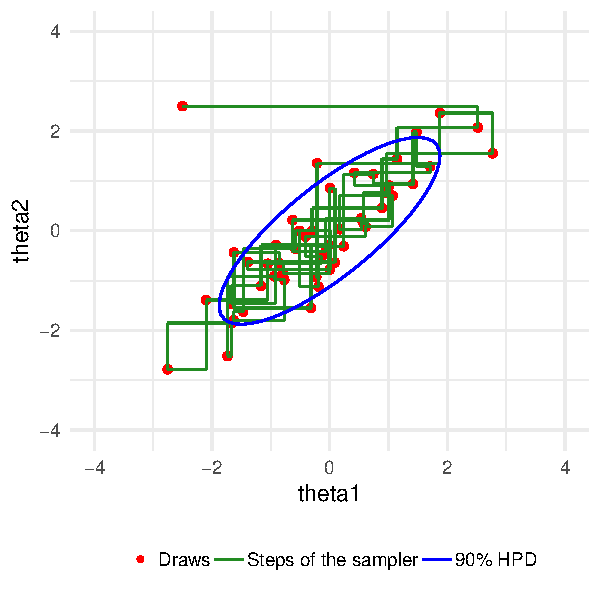
\includegraphics[width=5cm]{figs/Gibbs1.pdf}
     \end{center}
    \vspace{-.5\baselineskip}
     \begin{center}
       \href{https://github.com/MansMeg/BSDA/blob/main/lectures/L5/figs/gibbs_example.gif}{demo}
     \end{center}
\end{frame}

% TODO: Add example of a Gibbs sampling algorithm here (in math). Derive the conditional distributions

\begin{frame}

\frametitle{ Gibbs sampling}

  \vspace{-0.5\baselineskip}
  \begin{itemize}
  \item With {\it conditionally} conjugate priors, the sampling from
    the conditional distributions is easy for wide range of models
  \item<2-> BUGS / WinBUGS / OpenBUGS / JAGS
  \item<3-> No algorithm parameters to tune
  \item<4-> For not so easy conditionals, use  e.g. inverse-CDF
  \item<5-> Several parameters can be updated in blocks ({\em blocking})
  \item<6-> Slow if parameters are highly dependent in the posterior...
  \end{itemize}

\end{frame}

\begin{frame}
\frametitle{Gibbs sampling}

    \vspace{-.5\baselineskip}
     \begin{center}
       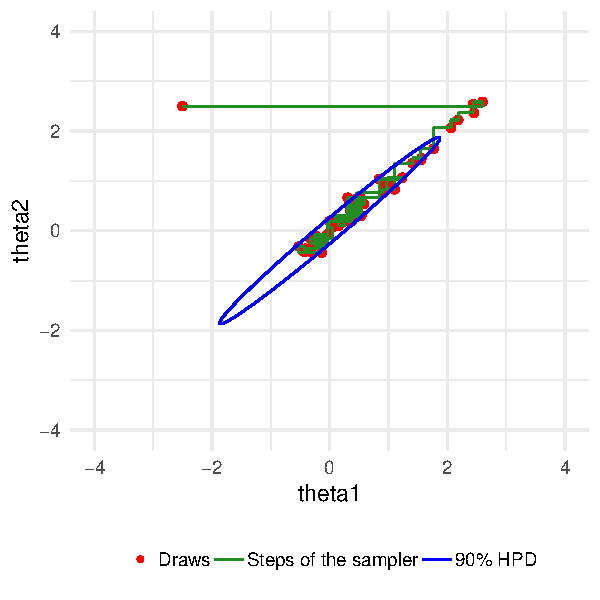
\includegraphics[width=5cm]{figs/Gibbs2.pdf}
     \end{center}
    \vspace{-.5\baselineskip}
     \begin{center}
       \href{https://github.com/MansMeg/BSDA/blob/main/lectures/L5/figs/gibbs_example_correlated.gif}{demo}
     \end{center}
\end{frame}

\subsection{Metropolis-Hastings}
%\frame{\sectionpage}

\begin{frame}

\frametitle{Sampling conditional vs joint}

  \begin{itemize}
  \item How about sampling $\theta$ jointly?
    \begin{itemize}
    \item e.g. it is easy to sample from multivariate normal
    \end{itemize}
    \item<2-> Can we use that to form a Markov chain?
  \end{itemize}

\end{frame}




\begin{frame}

\frametitle{The Metropolis algorithm}

  \begin{itemize}
  \item Algorithm
    \begin{itemize}
      \item[1.] starting point $\theta^0$
      \item[2.] $t=1,2,\ldots$
        \begin{itemize}
        \item[(a)] pick a proposal $\theta^{*}$ from a {\color{uured} proposal distribution}
          $J_t(\theta^{*}|\theta_{t-1})$. \\
          Proposal distribution has to be symmetric, i.e.\\
          $J_t(\theta_a|\theta_b)=J_t(\theta_b|\theta_a)$, for all
          $\theta_a,\theta_b$
        \item<2->[(b)] calculate acceptance ratio
          \begin{equation*}
            r=\frac{p(\theta^{*}|y)}{p(\theta_{t-1}|y)}
          \end{equation*}
          \vspace{-6mm}
        \item<3->[(c)] set
          \begin{equation*}
            \theta_t=
            \begin{cases}
              \theta^{*} & \text{with probability $\min(r,1)$}\\
              \theta_{t-1} & \text{otherwise}
            \end{cases}
          \end{equation*}
          \uncover<4>{
          ie, if $p(\theta^{*}|y)>p(\theta_{t-1}|y)$ accept the proposal always \\
          \hspace{0.4cm}and otherwise accept the proposal with probability $r$}
      \end{itemize}
      \vspace{-1.5\baselineskip}
    \item<5-> rejection of a proposal increments the time $t$ also by one\\
      ie, the new state is the same as previous
      \item<6-> step c is executed by generating a random number from
        $\U(0,1)$
      \item<7-> $p(\theta^*|y)$ and $p(\theta_{t-1}|y)$ have the same
        normalization terms, and thus instead of $p(\cdot|y)$,
        unnormalized $q(\cdot|y)$ can be used, { \color{uured} as the normalization terms cancel out}!
    \end{itemize}
  \end{itemize}

\end{frame}

\begin{frame}

\frametitle{ Metropolis algorithm}

  \begin{itemize}
  \item Example: one bivariate observation $(y_1,y_2)$
    \begin{itemize}
    \item bivariate normal distribution with unknown mean and known
      covariance
       \begin{equation*}
         \left.
         \begin{pmatrix}
           \theta_1\\
           \theta_2
         \end{pmatrix}
         \right| y \sim
         \N\left(
           \begin{pmatrix}
             y_1\\
             y_2
           \end{pmatrix},
           \begin{pmatrix}
             1 & \rho\\
             \rho & 1
         \end{pmatrix}
       \right)
       \end{equation*}
     \item proposal distribution
       $J_t(\theta^{*}|\theta_{t-1})=\N(\theta^{*}|\theta_{t-1},\sigma_p^2)$
     \end{itemize}
   \end{itemize}

  \center
  \href{https://chi-feng.github.io/mcmc-demo/app.html?algorithm=RandomWalkMH&target=standard}{demo}

\end{frame}

 \begin{frame}

\frametitle{Why Metropolis algorithm works}

  \begin{itemize}
  \item Intuitively more draws from the higher density areas as
    jumps to higher density are always accepted and only some of the
    jumps to the lower density are accepted
    \vspace{5mm}
    \pause
  \item Theoretically
    \begin{itemize}
    \item[1.] Prove that simulated series is a Markov chain
      which has unique stationary distribution
    \item[2.] Prove that this stationary distribution is the desired target distribution
    \end{itemize}
\end{itemize}

\end{frame}

\begin{frame}

\frametitle{Why Metropolis algorithm works}

  \begin{itemize}
  \item[1.] Prove that simulated series is a Markov chain
    which has unique stationary distribution
    \begin{itemize}
    \item[a)] irreducible
      \begin{itemize}
      \item<2->[=] positive probability of eventually reaching any
        state from any other state
      \end{itemize}
    \item[b)] aperiodic
      \begin{itemize}
      \item<3->[=] aperiodic (return times are not periodic)
      \item<3->[-] holds for a random walk on any proper distribution (except for trivial exceptions)
      \end{itemize}
    \item[c)] recurrent / not transient
      \begin{itemize}
      \item<4->[=] probability to return to a state $i$ is 1 as $T\rightarrow \infty$
      \item<4->[-] holds for a random walk on any proper distribution (except for trivial exceptions)
      \end{itemize}
    \end{itemize}
  \end{itemize}

\end{frame}


\begin{frame}

\frametitle{ Why Metropolis algorithm works}

  \begin{itemize}
  \item[2.] Prove that this stationary distribution is the desired target distribution $p(\theta|y)$
    \begin{itemize}
    \item[-] consider starting algorithm at time $t-1$ with a draw
      $\theta_{t-1} \sim p(\theta|y)$
    \item<2->[-] consider any two such points $\theta_a$ and $\theta_b$ drawn
      from $p(\theta|y)$ and labeled so that
      $p(\theta_b|y)\geq p(\theta_a|y)$
    \item<3->[-] the unconditional probability density of a transition from $\theta_a$ to $\theta_b$ is
      \vspace{-0.5\baselineskip}
      \begin{equation*}
        p(\theta_{t-1}=\theta_a,\theta_{t}=\theta_b)=
        p(\theta_a|y)J_t(\theta_b|\theta_a),
      \end{equation*}
      \vspace{-1\baselineskip}
    \item<4->[-] the unconditional probability density of a transition from $\theta_b$ to $\theta_a$ is
      \vspace{-0.5\baselineskip}
      \begin{eqnarray*}
        p(\theta_{t}=\theta_a,\theta_{t-1}=\theta_b) & = &
        p(\theta_b|y)J_t(\theta_a|\theta_b)\left(\frac{p(\theta_a|y)}{p(\theta_b|y)}\right)\\
        \pause &  = &  p(\theta_a|y)J_t(\theta_a|\theta_b),
      \end{eqnarray*}
      \uncover<5->{
      which is the same as the probability of transition from $\theta_a$ to $\theta_b$,
      since we have required that $J_t(\cdot|\cdot)$ is symmetric}
      \pause
    \item<6->[-] since their joint distribution is symmetric, $\theta_t$ and
      $\theta_{t-1}$ have the same marginal distributions, and so
      $p(\theta|y)$ is the stationary distribution of the Markov chain of $\theta$
    \end{itemize}
  \end{itemize}

\end{frame}

\begin{frame}

\frametitle{Metropolis-Hastings algorithm}

  \begin{itemize}
  \item Generalization of Metropolis algorithm for non-symmetric proposal distributions
    \begin{itemize}
    \item acceptance ratio includes ratio of proposal distributions
      \begin{equation*}
        r =
        \frac{p(\theta^{*}|y)/J_t(\theta^{*}|\theta_{t-1})}{p(\theta_{t-1}|y)/J_t(\theta_{t-1}|\theta^{*})} \pause =
        \frac{p(\theta^{*}|y)J_t(\theta_{t-1}|\theta^{*})}{p(\theta_{t-1}|y)J_t(\theta^{*}|\theta_{t-1})}
      \end{equation*}
    \end{itemize}
  \end{itemize}

\end{frame}

% \begin{frame}

% \frametitle{ Metropolis-Hastings algorithm}

%   \begin{itemize}
%   \item More efficient proposal distributions
%     \item e.g. Langevin-Hastings algorithm which uses gradient information to make proposals
%         \begin{itemize}
%         \item more likely to propose values with higher density
%         \end{itemize}
%   \end{itemize}

% \end{frame}

\begin{frame}

\frametitle{ Metropolis-Hastings algorithm}

  \begin{itemize}
  \item Ideal proposal distribution is the distribution itself
    \begin{itemize}
    \item $J(\theta^{*}|\theta)\equiv p(\theta^{*}|y)$ for all
      $\theta$
    \item acceptance probability is $1$
    \item independent draws
    \item not usually feasible
    \end{itemize}
  \item<2-> Good proposal distribution resembles the target distribution
    \begin{itemize}
    \item if the shape of the target distribution is unknown, usually
      normal or $t$ distribution is used
    \end{itemize}
  \item<3-> After the proposal distribution shape has been selected, it is important to select the scale
    \begin{itemize}
    \item small scale \\$\rightarrow$ many steps accepted, but the chain moves slowly due to small steps
    \item big scale \\$\rightarrow$ long steps proposed, but many of
      those rejected and again chain moves slowly
    \end{itemize}
  \href{https://chi-feng.github.io/mcmc-demo/app.html?algorithm=RandomWalkMH&target=standard}{demo}
  \item<4-> Generic rule for rejection rate is 60-90\% %(but depends on dimensionality and a specific algorithm variation)
\end{itemize}

\end{frame}

\begin{frame}

\frametitle{Gibbs sampling as a special case}

  \begin{itemize}
  \item Specific case of Metropolis-Hastings algorithm
    \begin{itemize}
    \item single updated (or blocked)
    \item proposal distribution is the conditional distribution\\
      $\rightarrow$ proposal and target distributions are same\\
      $\rightarrow$ acceptance probability is $1$
    \end{itemize}
  \end{itemize}

\end{frame}

\begin{frame}

\frametitle{ Metropolis}

  \begin{itemize}
  \item Usually doesn't scale well to high dimensions
    \begin{itemize}
    \item if the shape doesn't match the whole distribution, the efficiency drops
%    \item demo11\_2\\
      \vspace{1\baselineskip}
      \hspace{-1cm}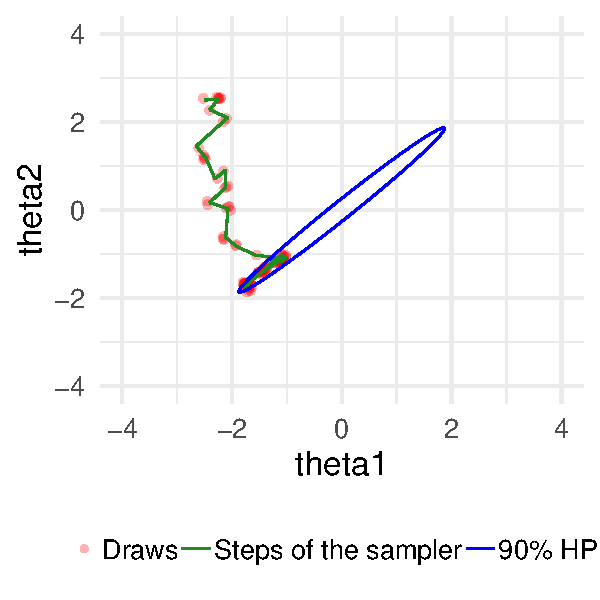
\includegraphics[width=4cm]{figs/Metrop2.pdf}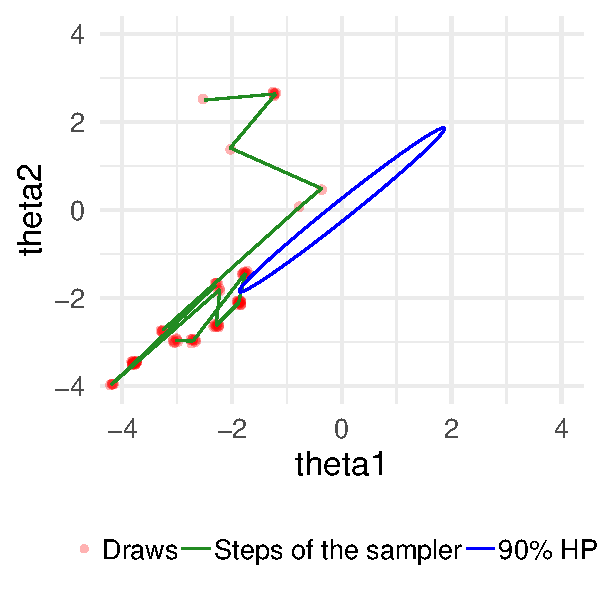
\includegraphics[width=4cm]{figs/Metrop3.pdf}
    \end{itemize}
  \end{itemize}

\end{frame}

\section{Diagnostics}
%\frame{\sectionpage}

\subsection{Warm-up}
%\frame{\sectionpage}

\begin{frame}

\frametitle{Warm-up}

  \begin{itemize}
  \item Asymptotically chain spends the $\alpha$\% of time where
    $\alpha$\% posterior mass is
    \uncover<2->{
      \begin{itemize}
      \item but in finite time the initial part of the Markov chain may be
        non-representative \\
        \hspace{2cm}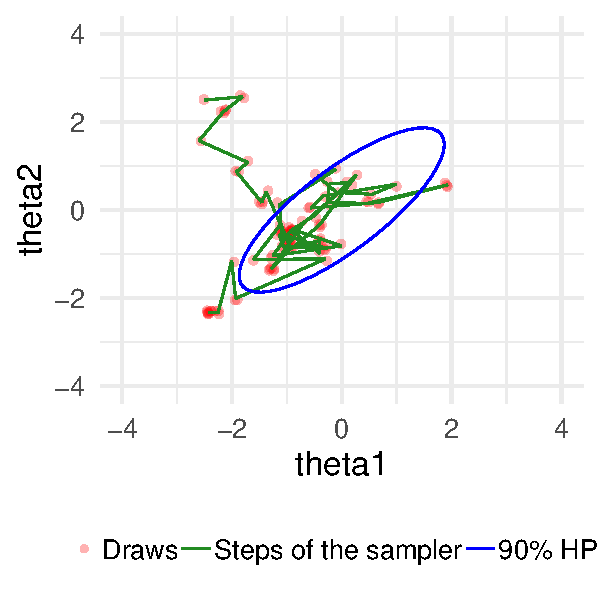
\includegraphics[width=4cm]{figs/Metrop1.pdf}
      \end{itemize}
      }
      \vspace{-.5\baselineskip}
    \item<3-> Warm-up period = (non-representative) draws from the beginning of the Markov chain
    \begin{itemize}
      \item remove warm-up before using samples for inference
      \item warm-up may include also phase for adapting algorithm parameters
      \end{itemize}
    \item<4-> Also called {\color{uured} burn-in}
  \end{itemize}

\end{frame}

\subsection{Convergence}
%\frame{\sectionpage}

\begin{frame}

\frametitle{Assesing convergence}

  \vspace{-0.5\baselineskip}
  \begin{itemize}
  \item Several Markov chains make convergence diagnostics easier
  \pause
    \item Start chains from different starting points -- preferably overdispersed
      \begin{center}
  \vspace{-0.5\baselineskip}
      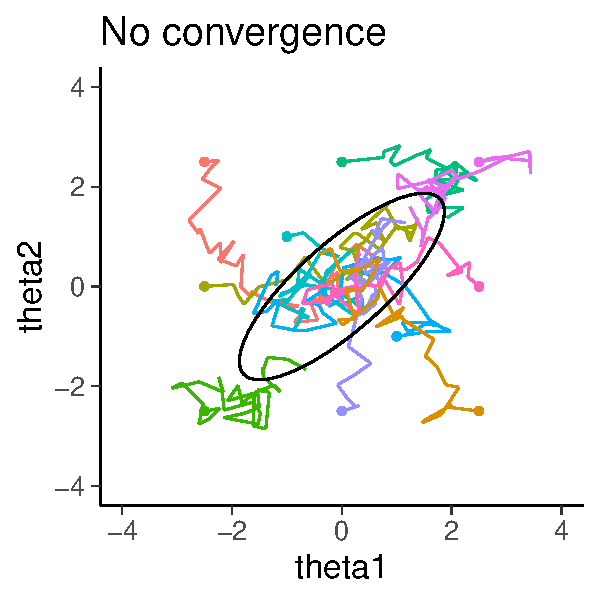
\includegraphics[width=6cm]{figs/10chains1.pdf}
    \end{center}
  \vspace{-0.5\baselineskip}
    \item<2-> Remove warm-up draws and run chains long enough
  \end{itemize}

\end{frame}

\begin{frame}

\frametitle{Several chains}

      \begin{center}
      \only<1>{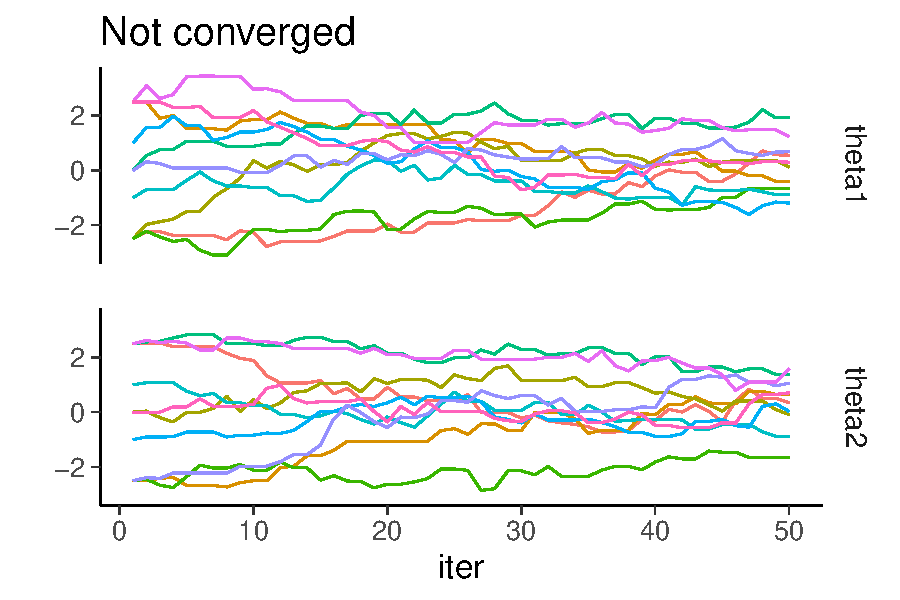
\includegraphics[width=8cm]{figs/10chains2.pdf}}
      \only<2->{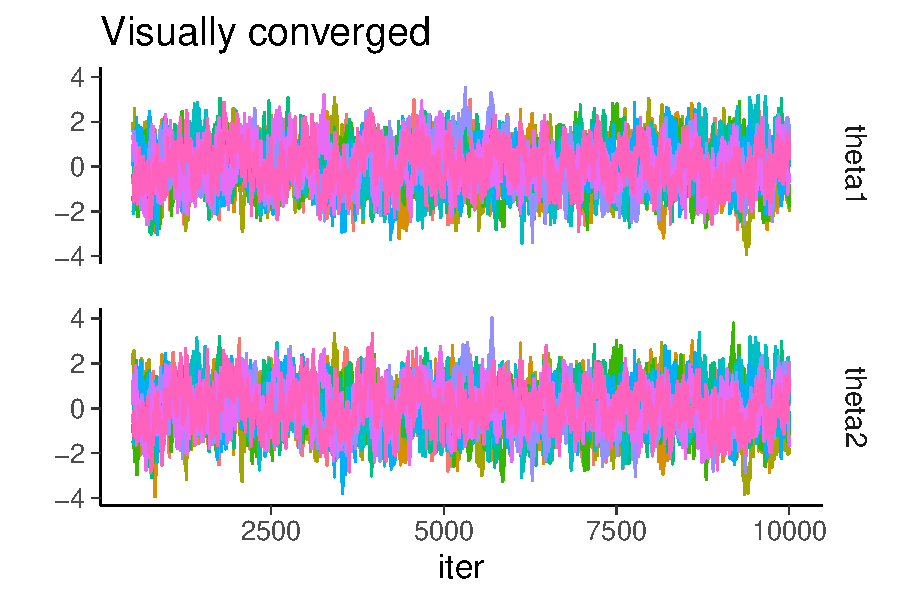
\includegraphics[width=8cm]{figs/10chains3.pdf}}\\
      \uncover<3->{Visual convergence check is not sufficient}
    \end{center}

\end{frame}



\begin{frame}[fragile]

\frametitle{ $\widehat{R}$: comparison of within and between variances of the chains}

  \begin{itemize}
  \item $\widehat{R}$ or {\color{uured} potential scale reduction factor} (PSRF)
  \item Compare means and variances of the chains\\
    \uncover<2->{W = within chain variance estimate\\
    var\_hat\_plus = total variance estimate\\}
    \vspace{1\baselineskip}
    \only<1>{\hspace{-0.5cm}\phantom{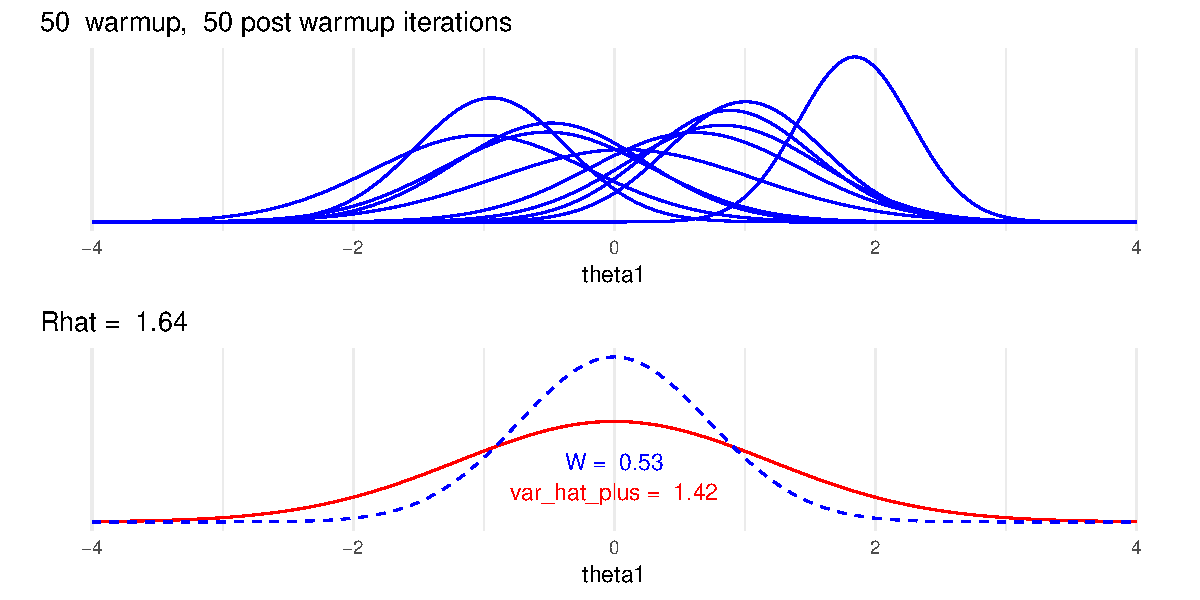
\includegraphics[width=8cm]{figs/10chains_rhat1.pdf}}}
    \only<2>{\hspace{-0.5cm}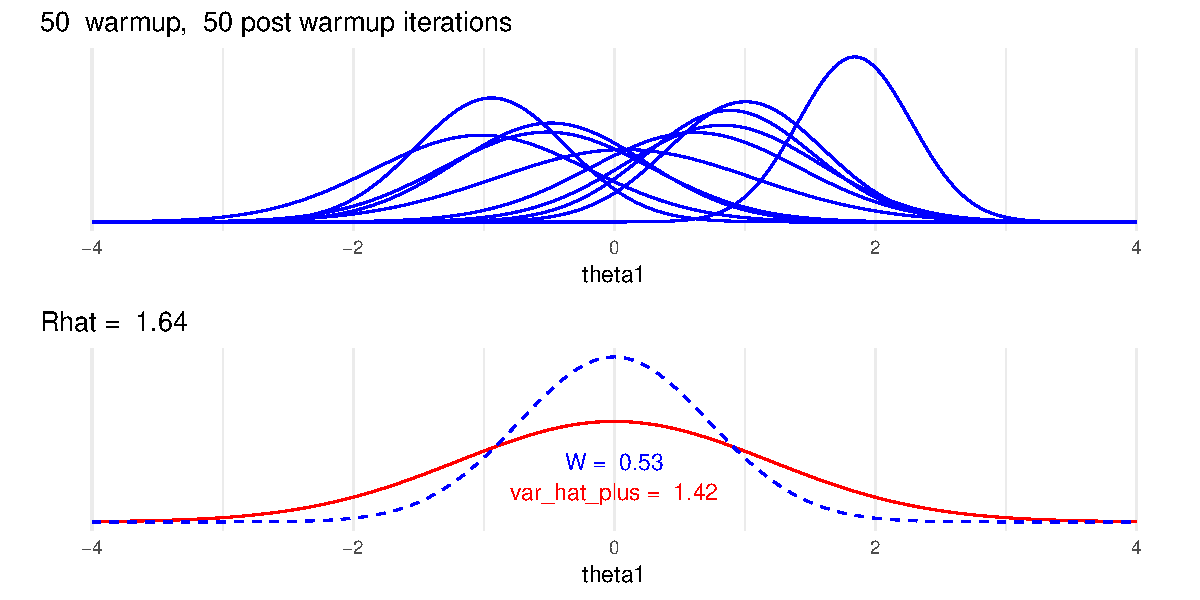
\includegraphics[width=8cm]{figs/10chains_rhat1.pdf}}
    \only<3>{\hspace{-0.5cm}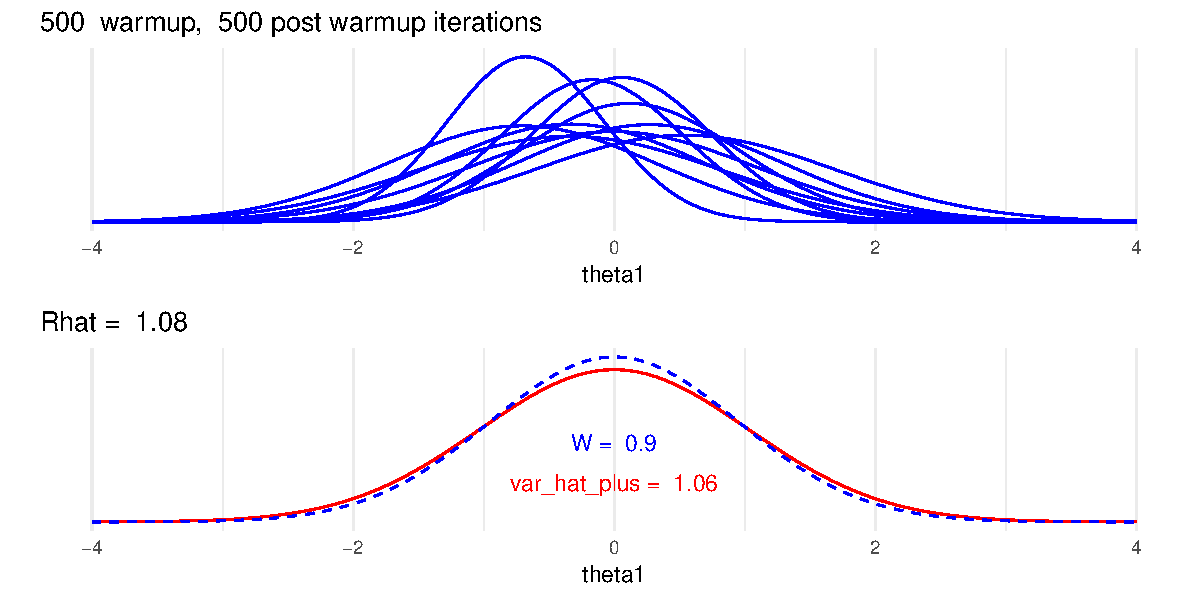
\includegraphics[width=8cm]{figs/10chains_rhat2.pdf}}
    \only<4>{\hspace{-0.5cm}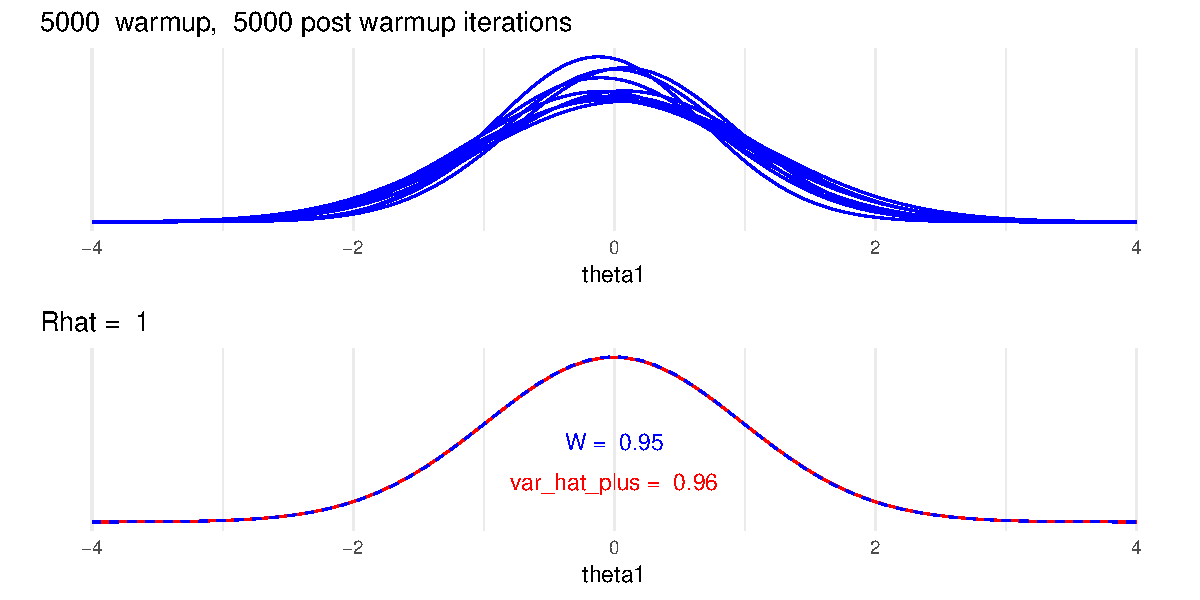
\includegraphics[width=8cm]{figs/10chains_rhat3.pdf}}
  \end{itemize}

\end{frame}

\begin{frame}

\frametitle{ $\widehat{R}$}

  \begin{itemize}
  \item $M$ chains, each having $N$ draws
  \item<2-> Within chains variance $W$
    \begin{equation*}
      W=\frac{1}{M}\sum_{m=1}^M s^2_m ,\text{ where }
      s^2_m=\frac{1}{N-1}\sum_{n=1}^N (\theta_{nm}-\bar{\theta}_{.m})^2
    \end{equation*}
  \item<3-> Between chains variance $B$
    \begin{align*}
      B&=\frac{N}{M-1}\sum_{m=1}^M
      (\bar{\theta}_{.m}-\bar{\theta}_{..})^2,\\
      &\text{ where } \bar{\theta}_{.m}=\frac{1}{N}\sum_{n=1}^N \theta_{nm}, \,
      \bar{\theta}_{..}=\frac{1}{M}\sum_{m=1}^M\bar{\theta}_{.m}
    \end{align*}
    %\vspace{-6mm}
    \begin{itemize}
      \item<4-> $B/N$ is variance of the means of the chains
    \end{itemize}
    \vspace{2mm}
  \item<5-> Estimate total variance
    $\var(\theta|y)$ as a weighted mean of $W$ and $B$
    \begin{equation*}
      \widehat{\var}^{+}(\theta|y) = \frac{N-1}{N}W+\frac{1}{N}B
    \end{equation*}
  \end{itemize}

\end{frame}


\begin{frame}

\frametitle{ $\widehat{R}$}

  \begin{itemize}
  \item Estimate total variance
    $\var(\theta|y)$ as a weighted mean of $W$ and $B$
    \begin{equation*}
      \widehat{\var}^{+}(\theta|y) = \frac{N-1}{N}W+\frac{1}{N}B
    \end{equation*}
    \vspace{-0.5\baselineskip}
    \begin{itemize}
    \item this \emph{overestimates} marginal posterior variance if the
      starting points are overdispersed
    \end{itemize}
    \vspace{0.5\baselineskip}
  \item<2-> Given finite $N$, $W$ \emph{underestimates} marginal posterior variance
    \begin{itemize}
    \item single chains have not yet visited all points in the distribution
    \item when $N\rightarrow\infty, \quad \E(W)\rightarrow \var(\theta|y)$
    \end{itemize}
    \vspace{0.5\baselineskip}
  \item<3-> As $\widehat{\var}^{+}(\theta|y)$ overestimates and $W$ underestimates,
    compute
    \begin{equation*}
      \widehat{R}=\sqrt{\frac{\widehat{\var}^{+}}{W}}
    \end{equation*}
\end{itemize}

\end{frame}


\begin{frame}[fragile]

\frametitle{ $\widehat{R}$}

  \begin{itemize}
  \item BDA3: $\widehat{R}$ aka {\em potential scale reduction factor} (PSRF)
  \item Compare means and variances of the chains\\
    W = within chain variance estimate\\
    var\_hat\_plus = total variance estimate\\
    \vspace{1\baselineskip}
    \only<1>{\hspace{-0.5cm}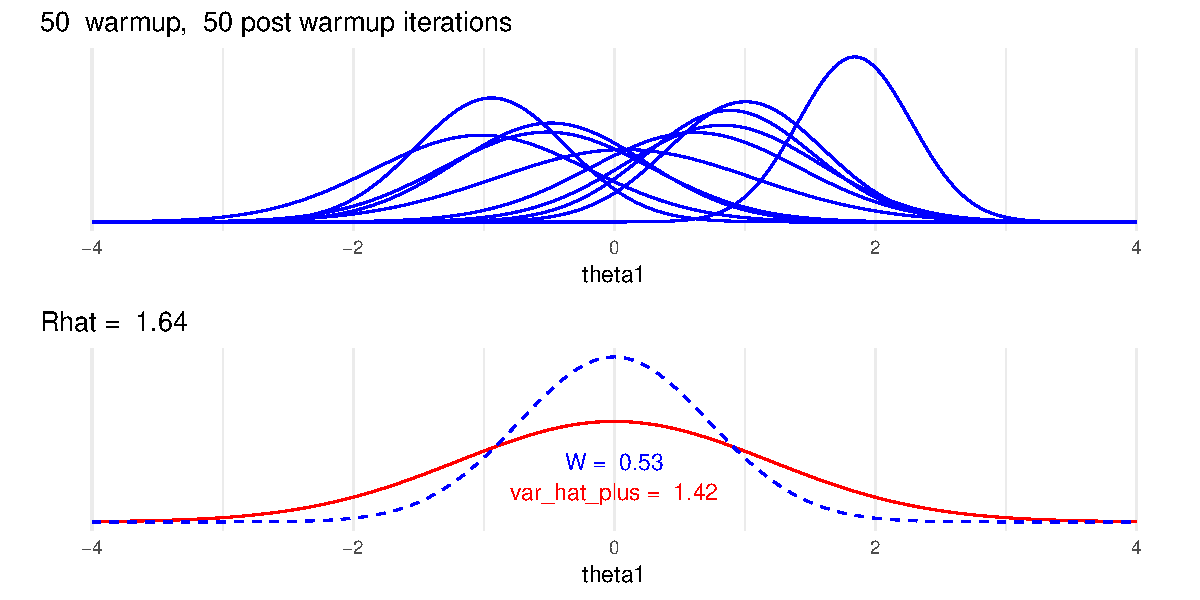
\includegraphics[width=8cm]{figs/10chains_rhat1.pdf}}
    \only<2>{\hspace{-0.5cm}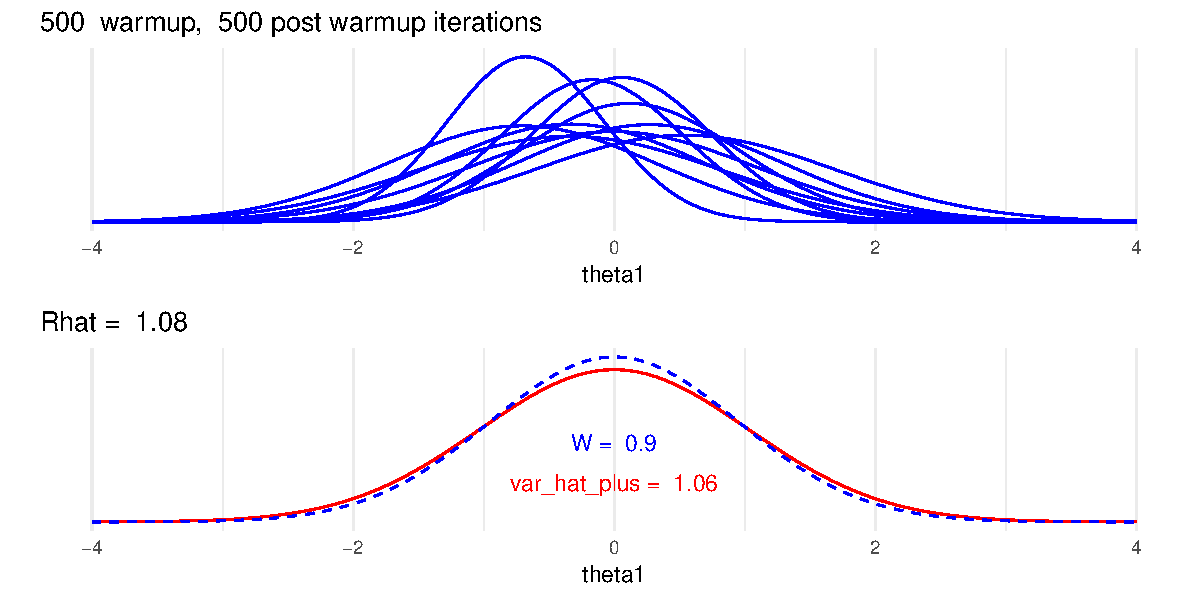
\includegraphics[width=8cm]{figs/10chains_rhat2.pdf}}
    \only<3>{\hspace{-0.5cm}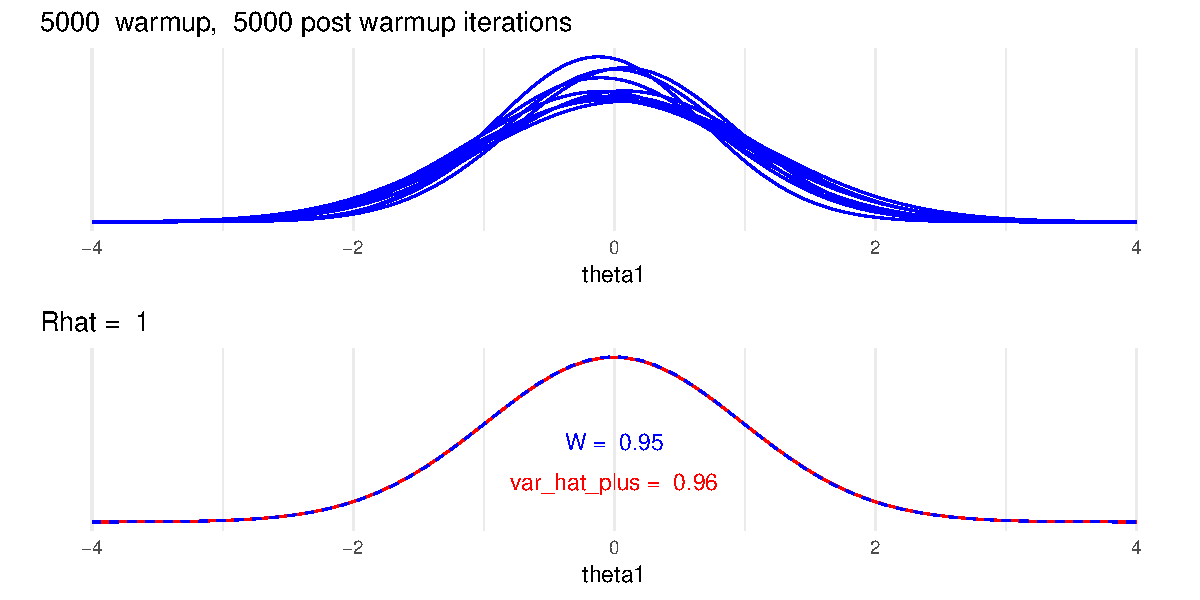
\includegraphics[width=8cm]{figs/10chains_rhat3.pdf}}
  \end{itemize}

\end{frame}

\begin{frame}

\frametitle{ $\widehat{R}$}

  \begin{equation*}
      \widehat{R}=\sqrt{\frac{\widehat{\var}^{+}}{W}}
    \end{equation*}
    \begin{itemize}
    \item<1-> Estimates how much the scale could reduce if $N\rightarrow\infty$
    \item<1-> $\widehat{R}\rightarrow 1$, when $N\rightarrow\infty$
    \item<1-> If $\widehat{R}$ is big (e.g., $R>1.01$), keep sampling
    \item<2-> If $\widehat{R}$ close to 1, it is still possible that chains have not converged
      \begin{itemize}
      \item if starting points were not overdispersed
      \item distribution far from normal (especially if infinite variance)
      \item just by chance when $N$ is finite
      \end{itemize}
    \end{itemize}

\end{frame}

\begin{frame}[fragile]

\frametitle{$\widehat{R}$}

  \begin{itemize}
  \item Additional $\widehat{R}$ methods to assess convergence
  \item Split-$\widehat{R}$
  \begin{itemize}
    \item Examines {\it mixing} and {\it stationarity} of chains
    \item To examine stationarity chains are split to two parts: compare means and variances of the split chains
  \end{itemize}
  \pause
  \item Rank normalized $\widehat{R}$
  \begin{itemize}
    \item Does not requires that the target distribution has finite mean and variance
  \end{itemize}
  \end{itemize}

\end{frame}


\subsection{$S_\text{eff}$, MCSE, and autocorrelation}
%\frame{\sectionpage}


\begin{frame}

\frametitle{MCMC draws are dependent}

  \begin{itemize}
    \item Monte Carlo estimates still valid (central limit theorem)
      \begin{align*}
        E_{\color{blue} p(\theta|y)}[f(\theta)] \approx \frac{1}{S} \sum_{s=1}^S f(\theta^{(s)})
      \end{align*}
    \item Estimation of Monte Carlo error is more difficult
      \begin{itemize}
        \item evaluation of {\it effective} sample size, $S_\text{eff}$.
      \end{itemize}
    \end{itemize}
\end{frame}

\begin{frame}

\frametitle{MCMC Autocorrelation}

  \begin{itemize}
  \item Auto correlation function
    \begin{itemize}
    \item describes the correlation given a certain lag
    \item can be used to compare efficiency of MCMC methods
    \end{itemize}
  \end{itemize}
%\vspace{.5cm}
%   \begin{center}
%       \includegraphics[scale=.8,clip]{kuva11_1}
%   \end{center}
\end{frame}

\begin{frame}

\frametitle{Autocorrelation}

  \vspace{-0.5\baselineskip}
  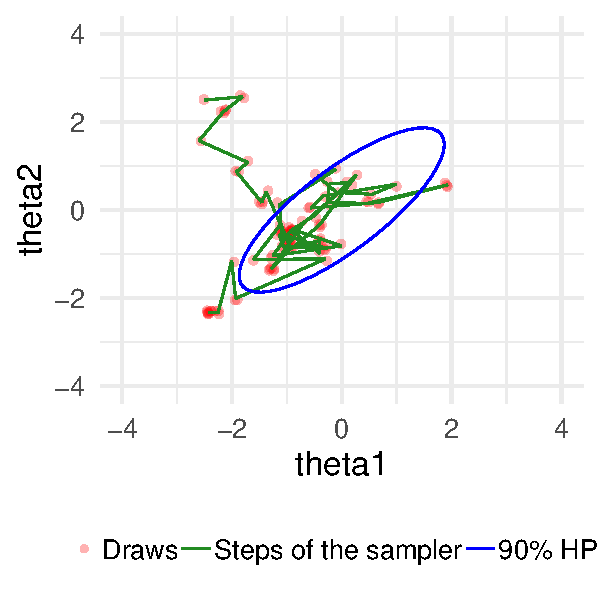
\includegraphics[width=4cm]{figs/Metrop1.pdf}
  \uncover<2->{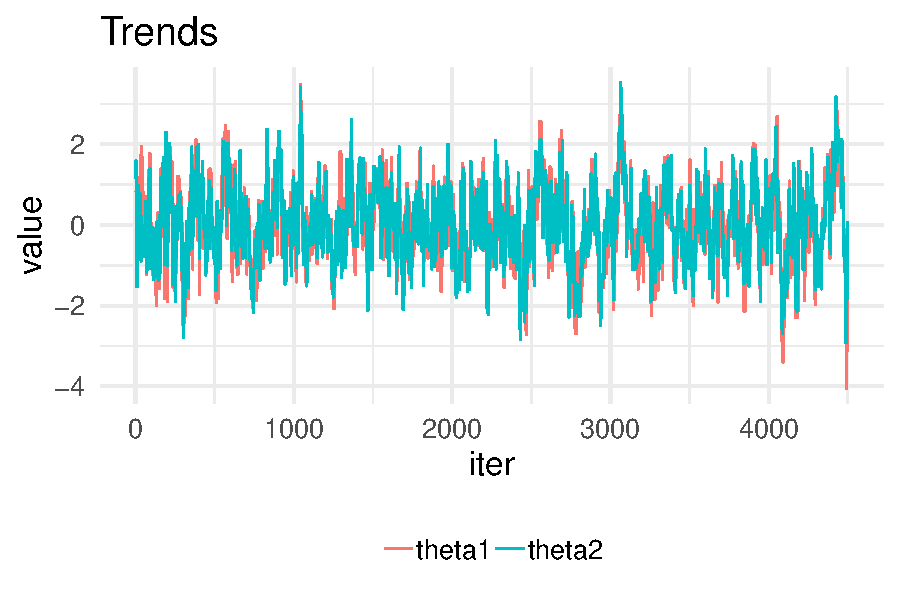
\includegraphics[width=5cm]{figs/Metrop1trace.pdf}\\}
  \uncover<3->{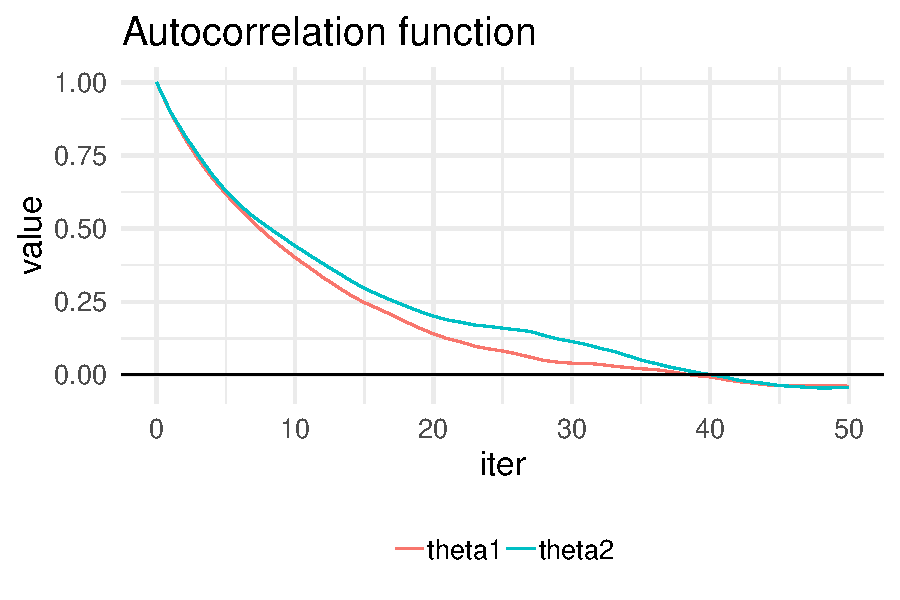
\includegraphics[width=5cm]{figs/Metrop1acf.pdf}}

\end{frame}

\begin{frame}

\frametitle{Autocorrelation}

  \vspace{-0.5\baselineskip}
  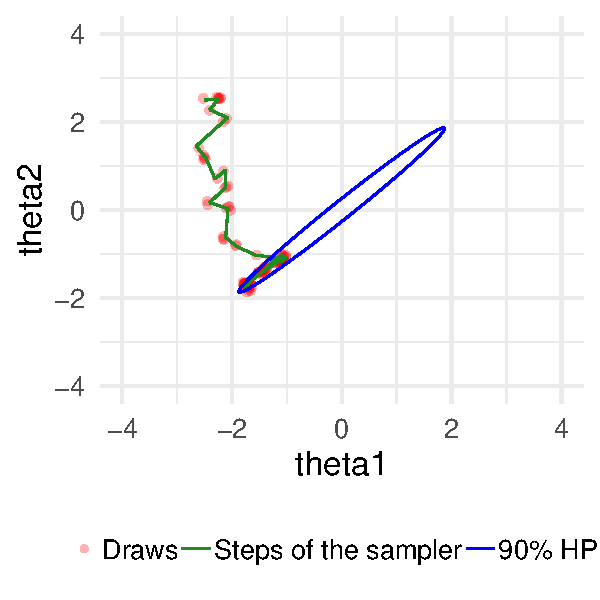
\includegraphics[width=4cm]{figs/Metrop2.pdf}
  {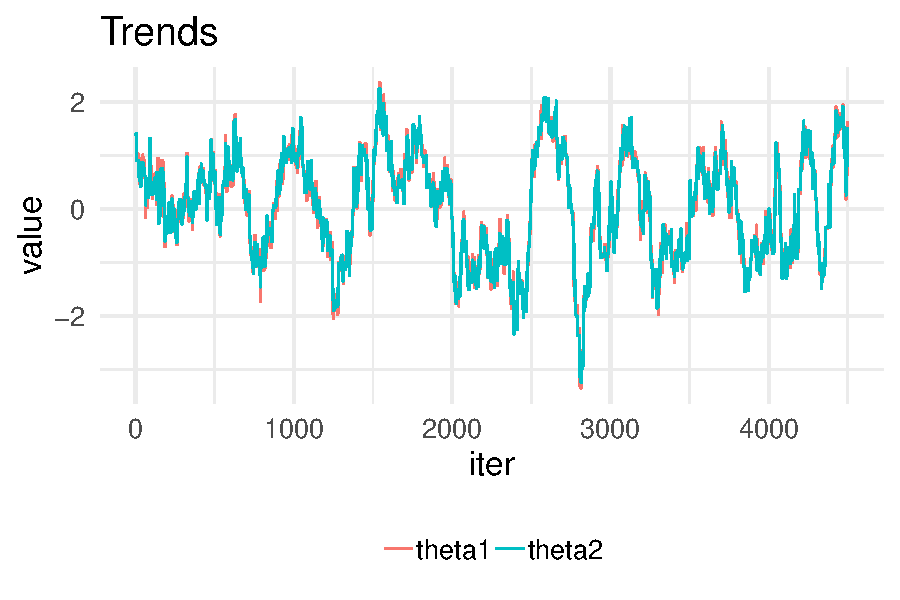
\includegraphics[width=5cm]{figs/Metrop2trace.pdf}\\}
  {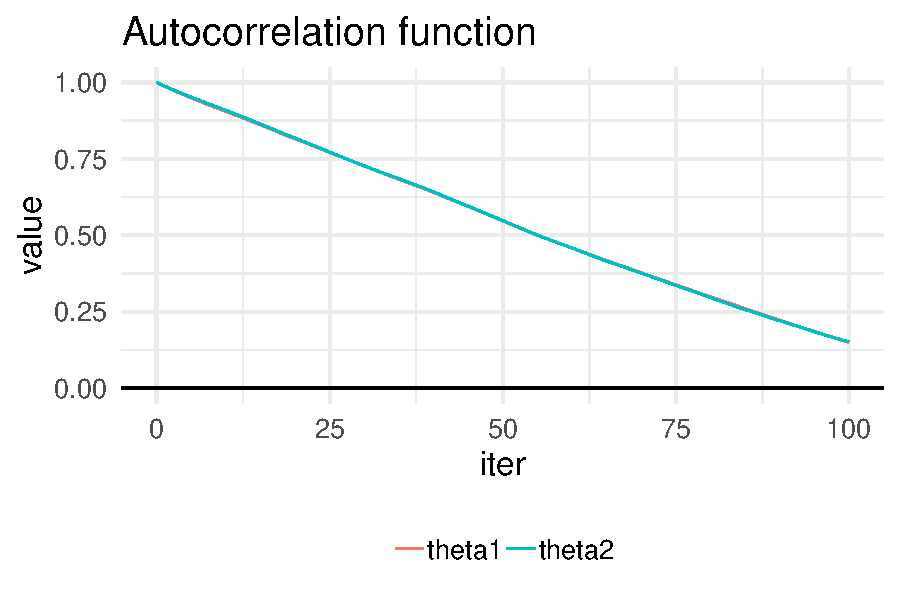
\includegraphics[width=5cm]{figs/Metrop2acf.pdf}}

\end{frame}

\begin{frame}

\frametitle{Autocorrelation}

  \vspace{-0.5\baselineskip}
  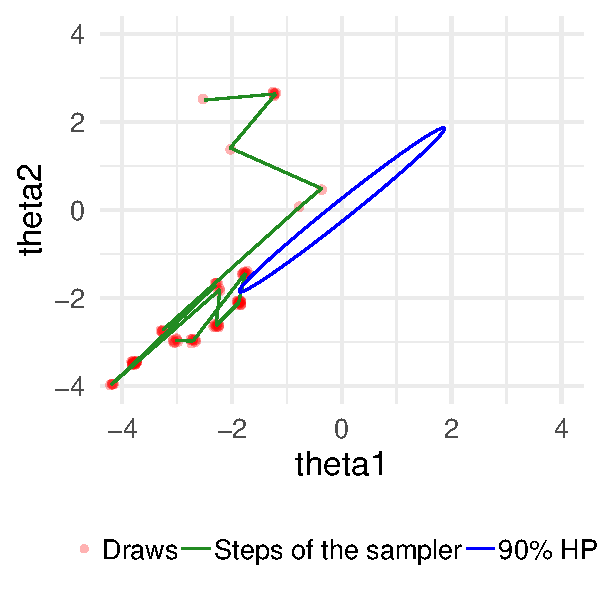
\includegraphics[width=4cm]{figs/Metrop3.pdf}
  {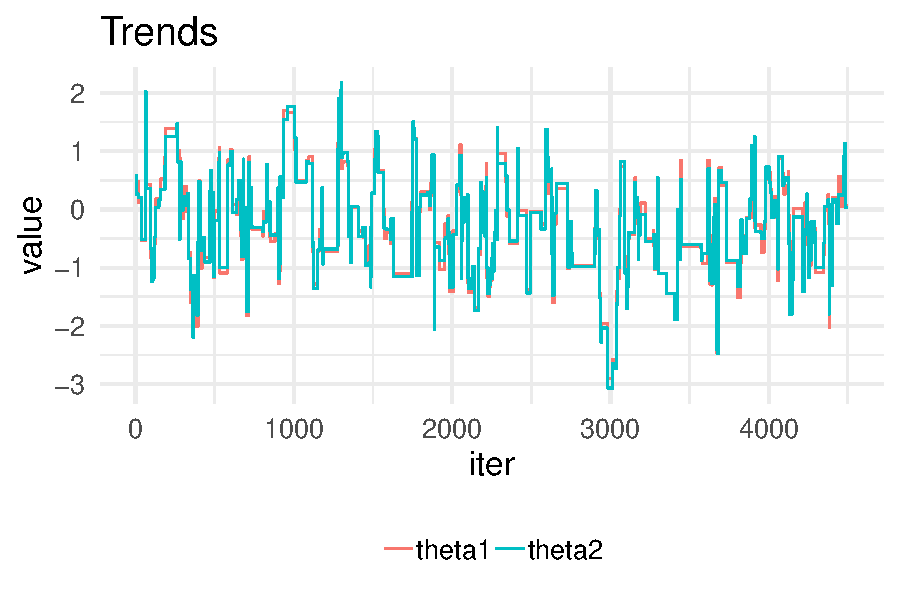
\includegraphics[width=5cm]{figs/Metrop3trace.pdf}\\}
  {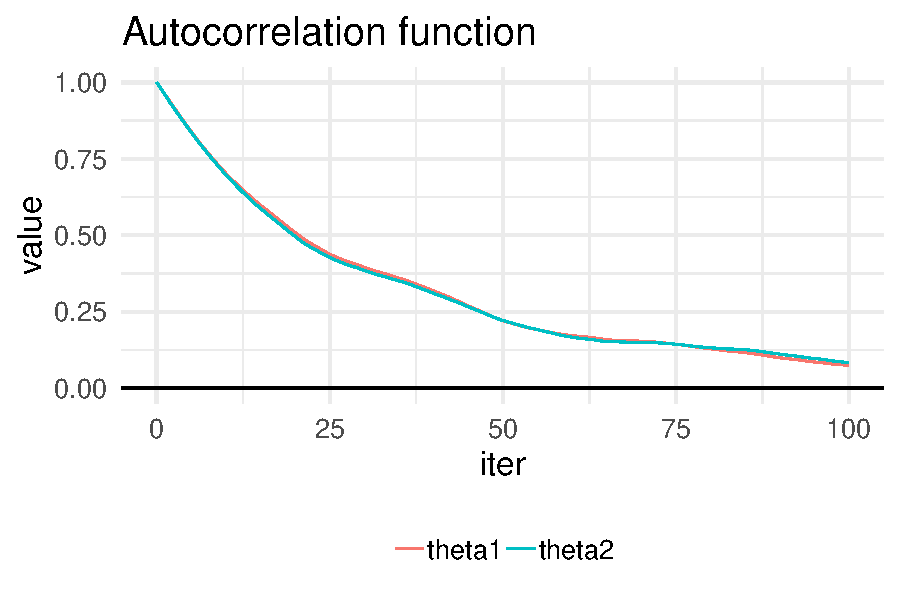
\includegraphics[width=5cm]{figs/Metrop3acf.pdf}}

\end{frame}

\begin{frame}

\frametitle{Autocorrelation}

  \begin{itemize}
  \item The autocorrleation can be used to estimate Monte Carlo error in case of MCMC
  \item For expectation $\bar{\theta}$
    \begin{equation*}
      \Var[\bar{\theta}] = \frac{\sigma^2_\theta}{S_\text{eff}}
    \end{equation*}
    where $S_\text{eff}=S/\tau$, and $\tau$ is sum of autocorrelations
    \begin{itemize}
      \item<2-> $\tau$ describes how many dependent draws correspond to one independent draw
      \item<3-> Here $S=NM$ (in BDA3 $N=nm$ and $n_\text{eff}=N/\tau$)
      \item<4-> BDA3 focuses on $S_\text{eff}$ and not the Monte Carlo error directly
%        new R-hat paper discusses more about MCSEs for different quantities
    \end{itemize}
  \end{itemize}
\end{frame}

\begin{frame}

\frametitle{Autocorrelation}

  \begin{itemize}
  \item Estimation of the autocorrelation using several chains
    \begin{equation*}
      \hat{\rho}_n=1-\frac{W - \frac{1}{M}\sum_{m=1}^M \hat{\rho}_{n,m}}{2\widehat{\var}^{+}}
    \end{equation*}
    where $\hat{\rho}_{n,m}$ is autocorrelation at lag $n$ for chain $m$
%  \item<2-> This combines $\widehat{R}$ and autocorrelation estimates
%    \begin{itemize}
%    \item takes into account if the chains are not mixing (the chains have not converged)
%    \end{itemize}
  \item<2-> BDA3 has slightly different and less accurate equation. The
    above equation is used in Stan 2.18+
  \item<3-> Compared to a method which computes the autocorrelation
    from a single chain, the multi-chain estimate has smaller variance
 \end{itemize}
\end{frame}



\begin{frame}

\frametitle{Estimating $\tau$}

  \begin{itemize}
  \item Estimation of $\tau$
    \begin{align*}
      \tau = 1 + 2 \sum_{t=1}^\infty \hat{\rho}_t
    \end{align*}
    where $\hat{\rho}_t$ is empirical autocorrelation
    \begin{itemize}
    \item<2-> empirical autocorrelation function is noisy %and thus
%      estimate of $\tau$ is noisy
    \item<2-> noise is larger for longer lags (less observations)
    \item<3-> less noisy estimate is obtained by truncating
    \begin{align*}
      \hat{\tau} = 1 + 2 \sum_{t=1}^T \hat{\rho}_t
    \end{align*}
    \end{itemize}
%    \item<4-> As $\tau$ is estimated from a finite number of draws,
%      it's expectation is overoptimistic
%      \begin{itemize}
%      \item if $\hat{\tau}>MN/20$ then the estimate is unreliable
%
%      \end{itemize}
    \end{itemize}
\end{frame}

\begin{frame}

\frametitle{Geyer's adaptive window estimator of $\tau$}

  \begin{itemize}
  \item Truncation $T$ can be decided adaptively
    \begin{itemize}
    \item for stationary, irreducible, recurrent Markov chain
    \item let $\Gamma_m=\rho_{2m}+\rho_{2m+1}$, which is sum of two
      consequent autocorrelations
    \item $\Gamma_m$ is positive, decreasing and convex function of $m$
    \end{itemize}
    \vspace{0.5\baselineskip}
  \item<2-> Initial positive sequence estimator (Geyer's IPSE)
      \begin{itemize}
        \item Choose the largest $m$ so, that all values of the sequence
        $\hat{\Gamma}_1, \ldots, \hat{\Gamma}_m$ are positive
      \end{itemize}
  \vspace{0.5\baselineskip}
      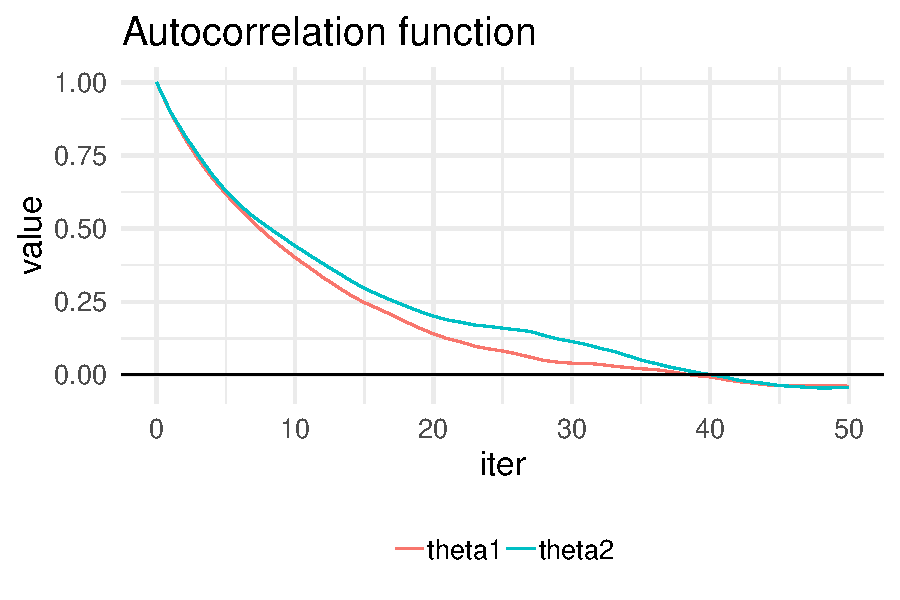
\includegraphics[width=6cm]{figs/Metrop1acf.pdf}
  \end{itemize}
\end{frame}

% Gibbs1 neff=252, N=2001
% Gibbs2 neff=12, N=2001, Rhat 1.11
% Metrop1 neff=194, N=5000
% Metrop2 neff=48, N=5000
% Metrop3 neff=81, N=5000

\begin{frame}

 \frametitle{Effective sample size, $S_\text{eff}$}

   Effective sample size $\ESS = S_\text{eff} \approx S/\hat{\tau}$\\
   \uncover<2->{
  \makebox[12cm][t]{
    \hspace{-.7cm}
     \begin{minipage}{12cm}
     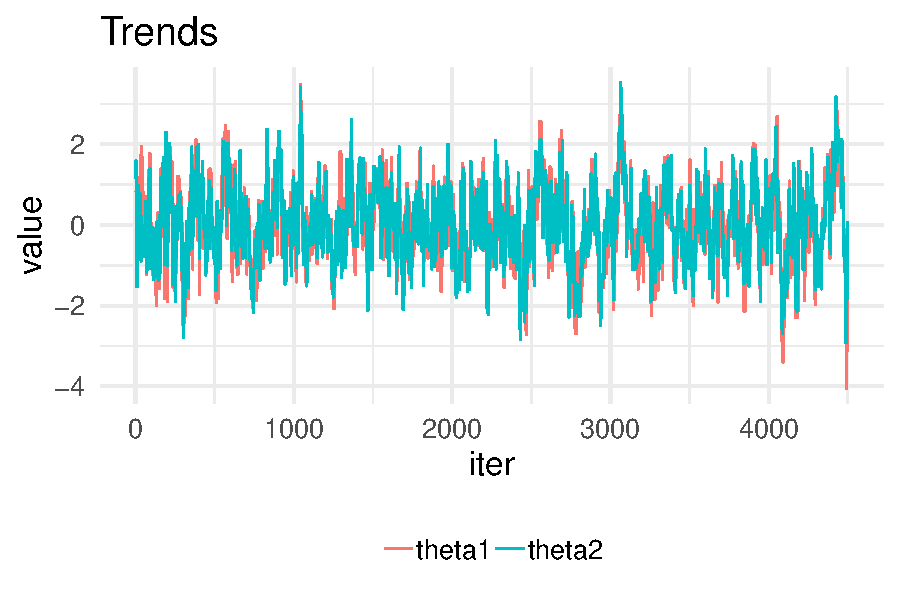
\includegraphics[width=5cm]{figs/Metrop1trace.pdf}
     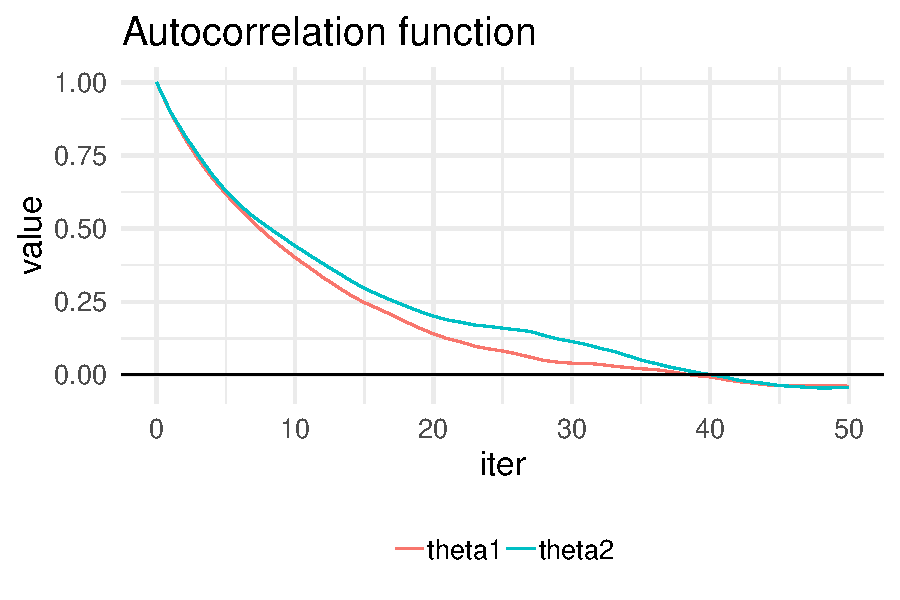
\includegraphics[width=5cm]{figs/Metrop1acf.pdf}\\
     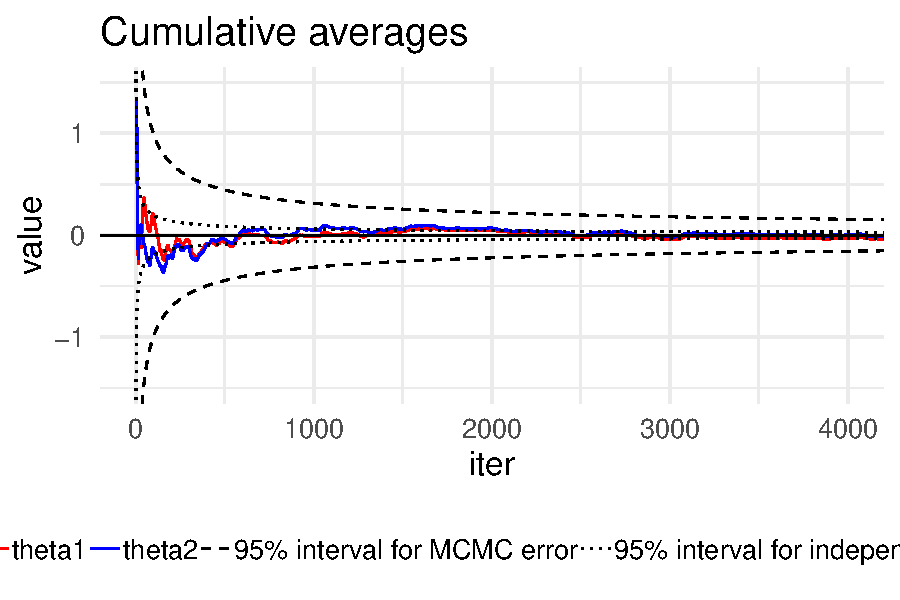
\includegraphics[width=5cm]{figs/Metrop1mcerr.pdf}
     \hspace{0cm}
     \begin{minipage}[t][4cm][t]{5cm}
       \vspace{-2.5cm}
       \begin{align*}
         \hat{\tau} & = 1 + 2 \sum_{t=1}^T \hat{\rho}_t\\
                 & \approx 24
       \end{align*}
     \end{minipage}
   \end{minipage}
   }
   }

\end{frame}

\begin{frame}

 \frametitle{ Effective sample size}

   Effective sample size $\ESS = S_\text{eff} \approx S/\hat{\tau}$\\
  \makebox[12cm][t]{
    \hspace{-.7cm}
     \begin{minipage}{12cm}
     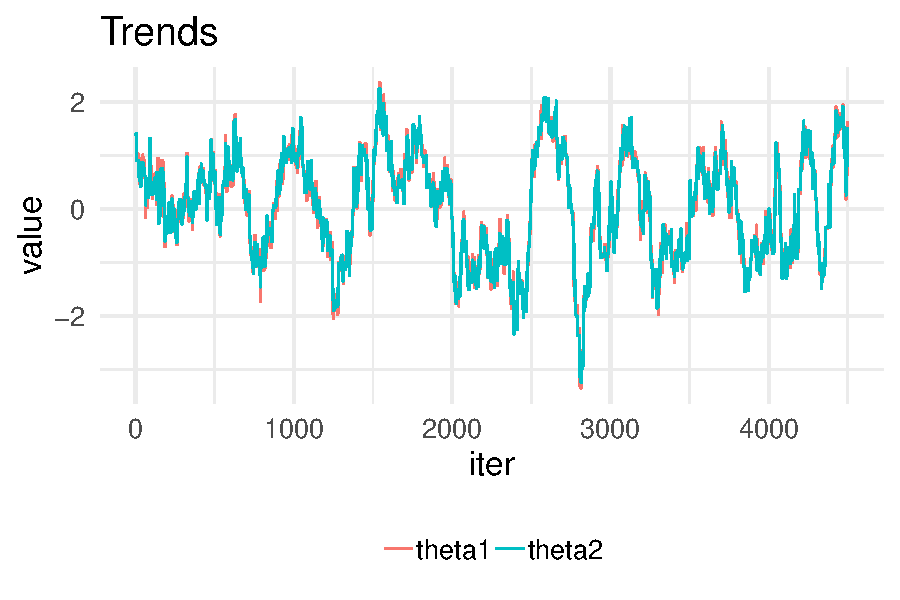
\includegraphics[width=6cm]{figs/Metrop2trace.pdf}
     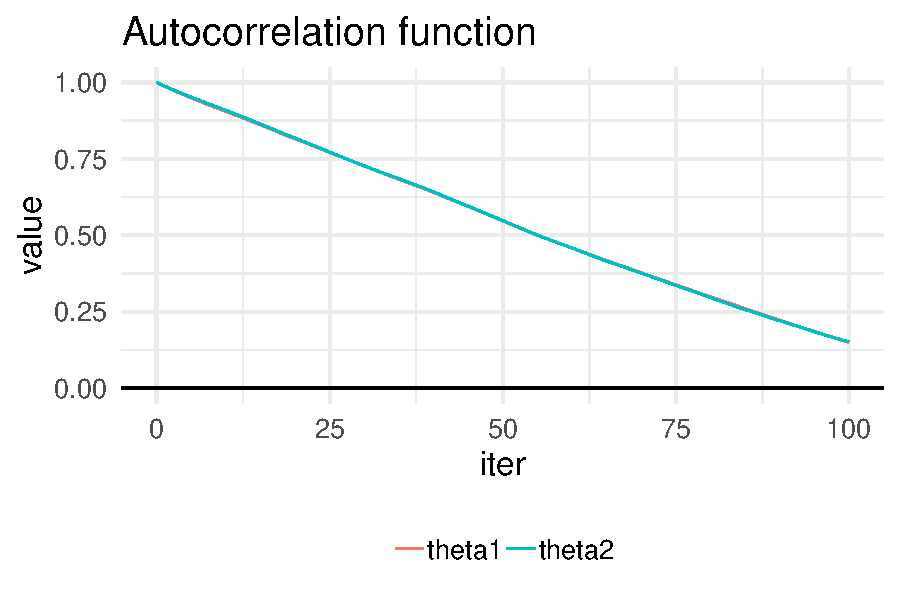
\includegraphics[width=6cm]{figs/Metrop2acf.pdf}\\
     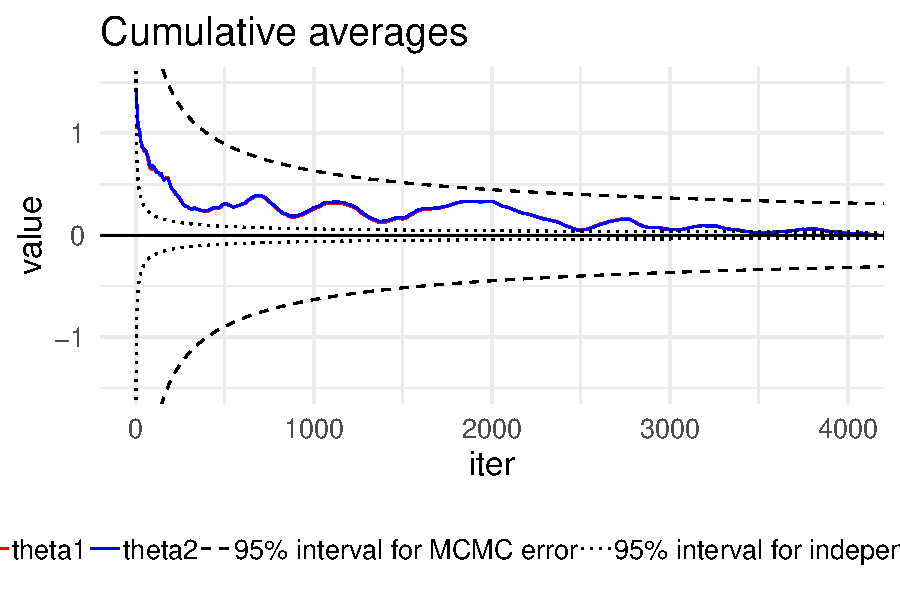
\includegraphics[width=6cm]{figs/Metrop2mcerr.pdf}
     \hspace{0cm}
     \begin{minipage}[t][4cm][t]{6cm}
       \vspace{-3.5cm}
       \begin{align*}
         \hat{\tau} & = 1 + 2 \sum_{t=1}^T \hat{\rho}_t\\
                 & \approx 104
       \end{align*}
     \end{minipage}
   \end{minipage}
   }

\end{frame}

\begin{frame}

 \frametitle{ Effective sample size}

   Effective sample size $\ESS = S_\text{eff} \approx S/\hat{\tau}$\\
  \makebox[12cm][t]{
    \hspace{-.7cm}
     \begin{minipage}{12cm}
     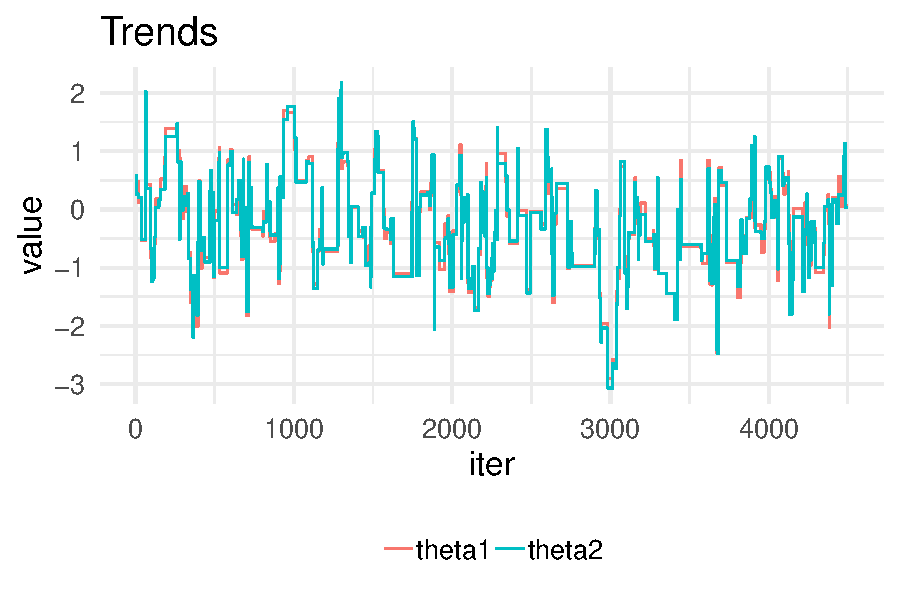
\includegraphics[width=6cm]{figs/Metrop3trace.pdf}
     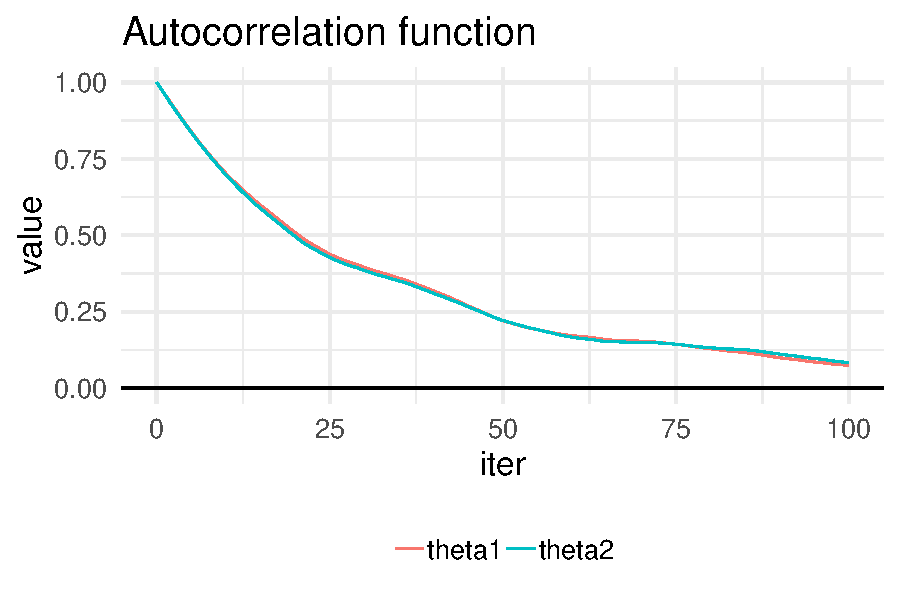
\includegraphics[width=6cm]{figs/Metrop3acf.pdf}\\
     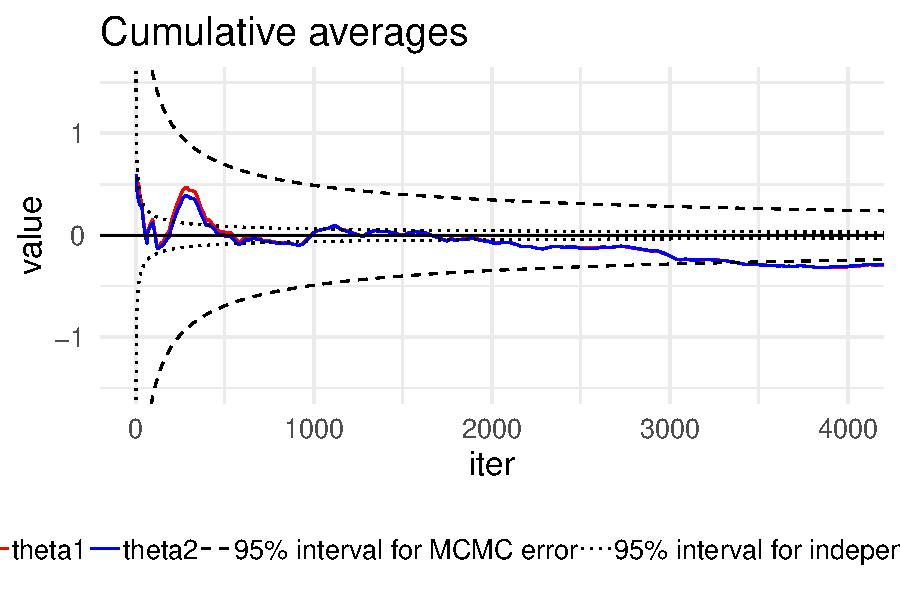
\includegraphics[width=6cm]{figs/Metrop3mcerr.pdf}
     \hspace{0cm}
     \begin{minipage}[t][4cm][t]{6cm}
       \vspace{-3.5cm}
       \begin{align*}
         \hat{\tau} & = 1 + 2 \sum_{t=1}^T \hat{\rho}_t\\
                 & \approx 63
       \end{align*}
     \end{minipage}
   \end{minipage}
   }

\end{frame}

\begin{frame}

\frametitle{ Problematic distributions}

  \begin{itemize}
  \item<1-> Nonlinear dependencies
    \begin{itemize}
    \item optimal proposal depends on location
    \end{itemize}
  \item<2-> Funnels
    \begin{itemize}
    \item optimal proposal depends on location
    \end{itemize}
  \item<3-> Multimodal
    \begin{itemize}
    \item difficult to move from one mode to another
    \end{itemize}
  \item<4-> Long-tailed with non-finite variance and mean
    \begin{itemize}
    \item central limit theorem for expectations does not hold
    \end{itemize}
  \end{itemize}

\end{frame}

%%%%%%%%%%%%%%%%%%%%%%%%%%%%%%%%%%%%%%%%%%%%%%%%%%%%%%%%%%%%%%%%%%


\end{document}
